%%%% Version 5. Single-modality (surface EMG) revision of main_4.tex.
%%%%
%%%% Relative to v4:
%%%%   * The microphone is removed from the analysis entirely. It survives as one
%%%%     Methods paragraph (Section "The channel that is not analysed") recording that
%%%%     it was collected as an annotation aid and excluded on measured signal quality.
%%%%     The multimodal-fusion research question is gone with it.
%%%%   * The reported model is the EMG-only condition of the modality run, not the fused
%%%%     condition of the primary run. Every headline number changes accordingly.
%%%%   * The measurement-chain audit is promoted from a methodological aside to the
%%%%     paper's first research question, and the screening contrast that supports it is
%%%%     recomputed on the 28 EMG features alone so that no reported number reads the
%%%%     microphone, directly or through a feature.
%%%%   * The architecture question is reframed from "does this network beat three
%%%%     unrun deep baselines" to "does the learned wavelet representation beat
%%%%     hand-engineered band energies", which the archive can answer.
%%%%   * Three design constraints the archive can measure -- window length, trigger
%%%%     granularity, normalisation scope -- are promoted into the Results.
%%%%
%%%% Every reported number comes from one of these artifacts:
%%%%   outputs/runs/modality_and_no_chewing_20260810T020642_cead62e4  (emg_only conditions)
%%%%   outputs/screening/emg_only_filter_contrast.json                (RQ1 filter contrast)
%%%%   outputs/screening/emg_only_design.json                         (design constraints)
%%%%   outputs/screening/emg_only_contrast.json                       (RQ3 feature baselines)
%%%%   outputs/data_audit/7ebbcc8d74c0bbe0/                           (guards, sweeps, mains)
%%%%   outputs/benchmarks/benchmark.json                              (reference latencies)
%%%% Run-dependent figures live in Figures/v5/ so that main_4.tex still compiles.
\documentclass[pdflatex,sn-nature,iicol]{sn-jnl}

\usepackage{graphicx}
\usepackage{multirow}
\usepackage{amsmath,amssymb}
\usepackage{booktabs}
\usepackage{mathrsfs}
\usepackage[title]{appendix}
\usepackage{xcolor}
\usepackage{textcomp}
\usepackage{manyfoot}
\usepackage{indentfirst}

\graphicspath{{./}{figures/}{Figures/}}
\providecommand{\Description}[1]{}

\begin{document}

\title[Audited Surface-EMG Classification of Instructed Jaw Activities]{The Measurement Chain Outweighs the Model: Audited Surface-EMG Classification of Instructed Jaw Activities Relevant to Tooth-Contact Bruxism}

\author[1]{\fnm{Mohammad Hassan} \sur{Farhadi}}
\author[1]{\fnm{Ali} \sur{Rabiee}}
\author[1]{\fnm{Rahul} \sur{Singh}}
\author[2,3]{\fnm{Mariusz P.} \sur{Furmanek}}
\author*[1]{\fnm{Reza} \sur{Abiri}}\email{reza\_abiri@uri.edu}
\author*[4]{\fnm{Theodore A.} \sur{Walls}}\email{walls@uri.edu}

\affil[1]{\orgdiv{Department of Electrical, Computer, and Biomedical Engineering}, \orgname{University of Rhode Island}, \orgaddress{\city{Kingston}, \state{RI}, \country{United States}}}
\affil[2]{\orgdiv{Department of Physical Therapy}, \orgname{University of Rhode Island}, \orgaddress{\city{Kingston}, \state{RI}, \country{United States}}}
\affil[3]{\orgdiv{Institute of Sport Sciences, Academy of Physical Education in Katowice}, \orgaddress{\city{Katowice}, \country{Poland}}}
\affil[4]{\orgdiv{Department of Psychology}, \orgname{University of Rhode Island}, \orgaddress{\city{Kingston}, \state{RI}, \country{United States}}}

\abstract{Instrumental studies of masticatory-muscle activity are reported almost entirely through summary accuracies, and the measurement chain that produced them is rarely auditable. We show, on our own recordings, that this chain can outweigh every modelling choice made on top of it. A spectral audit of 100 awake laboratory recordings from five adults with a prior clinical diagnosis of bruxism found that the acquisition hardware had already suppressed the 60-Hz mains fundamental and that the surviving interference was harmonic: 62 recordings carried more than 30\% of their raw in-band electromyographic power within $\pm3$~Hz of a mains multiple, and in the five dedicated quiet-rest recordings that share reached 91.3--99.8\%. The conventional preprocessing recipe---notch the fundamental, then band-pass---removed the one frequency that was absent and passed everything that was present. Replacing it with a constant-width harmonic notch bank moved a matched nested leave-one-subject-out (LOSO) network from 43.5\% to 72.8\% participant-level macro-F1 on byte-identical windows, folds and labels---and two far simpler classifiers by 22 to 27 points over the same change---while cutting quiet-rest false alarms from 30.2\% to 6.1\% in that matched arm, eliminating all 20 participant pairs in which one person's resting EMG had exceeded another person's active EMG, and reducing the between-participant amplitude spread from $5.07\times$ to $2.97\times$. Two participants who had been unclassifiable, at 5.4\% and 18.1\% macro-F1, moved into the normal range: what had looked like severe between-participant heterogeneity was largely interference. On the corrected signal, a compact single-branch wavelet convolutional neural network with 5,901 parameters (23.1~KiB) separated quiet rest, jaw movement, clenching, instructed grinding, and chewing at 81.7\% accuracy, 72.0\% macro-F1 and a macro one-vs-rest ROC--AUC of 0.958, averaged over five held-out participants and three seeds under leakage-free nested LOSO. Quiet rest was the best-recalled class (91.4\% recall, AUC 0.958); collapsing the predictions into instructed clenching/grinding versus rest/movement/chewing gave 92.5\% accuracy, an F1 of 85.5\% and an AUC of 0.970, with 7.7\% of quiet-rest windows on the tooth-contact side. The learned representation beat hand-engineered band energies on identical windows and folds by 8.1 points of macro-F1 against logistic regression and 10.6 against gradient boosting---an advantage that did not exist before the filter correction. Two further constraints proved larger than the architecture: normalisation scope was worth 9.1 points of screening macro-F1, and macro-F1 rose monotonically from 0.730 to 0.804 as temporal context grew from 1.0 to 5.5~s, so the 1-second window is a constraint of this design rather than a tuned parameter. A microphone was also recorded, as an annotation aid; a channel-integrity audit found it unusable and it is not analysed. These results establish technical feasibility for this five-participant dataset and, more durably, a reporting practice: publish a measured interference statistic beside every accuracy, and draw filter responses over the measured spectrum of the recordings rather than alone.}

\keywords{Jaw-activity classification, Surface electromyography, Convolutional neural networks, Wavelet decomposition, Powerline interference, Signal-quality audit, Measurement validity, Leave-one-subject-out validation}

\maketitle

\section{Introduction}

Instrumental assessment of masticatory-muscle activity outside the clinic is a sensing and classification problem before it is anything else. Surface EMG measures masticatory activation directly and is the standard modality for ambulatory recording~\cite{raez2006techniques,colonna2023electromyographic}, but it responds similarly to functional and non-functional activity: clenching, grinding, and chewing all produce sustained or bursting masseter and temporalis activation, and a one-second window of one can resemble a window of another. Whether a compact learned model can separate those conditions from each other and from quiet rest, on participants it has never seen, is one of the questions this paper measures.

It is not the first one. Studies in this area are reported almost exclusively through summary accuracies, and the measurement chain that produced those accuracies is rarely auditable. During the preparation of this analysis, a spectral audit of our own recordings showed that the conventional preprocessing recipe applied to them---notch the mains fundamental, then band-pass---removed the one frequency the acquisition hardware had already suppressed and left the mains \emph{harmonics}, which carried the overwhelming majority of the in-band power, entirely intact. A filter-response plot of that chain looks textbook-correct. Nothing in the pipeline was untested, unversioned, or irreproducible; the defect was invisible because no figure had ever placed the filter response over the measured spectrum of the data.

Correcting it changed the results by more than every other intervention we evaluated combined. That outcome is the organising claim of this paper, and it is stated first because it reorders what is worth reporting. A classifier trained through a defective channel can appear to work while separating interference rather than physiology, and leave-one-subject-out evaluation is precisely the protocol that then reports the consequence as poor generalisation across people. We therefore report the audit, the correction, its measured effect on classification, and only then the classifier that runs on the corrected signal.

\subsection*{Scope}

Two scope statements follow from current terminology and are made here once. International consensus defines bruxism as masticatory-muscle activity that may involve clenching or grinding with tooth contact, or bracing and thrusting without it, and distinguishes sleep from awake manifestations~\cite{lobbezoo2018international,verhoeff2025definitions}. Tooth contact is therefore neither necessary for all bruxism activities nor sufficient to establish that an observed activity is bruxism. Second, every activity analysed here was performed on instruction in a laboratory: the class names used below---rest, movement, clenching, grinding, and chewing---denote experimental conditions, and a classifier that separates them is not a diagnostic device. Both points constrain how the numbers in this paper may be read, and neither is revisited later. The study does not evaluate spontaneous awake bruxism, sleep bruxism, severity, or treatment response.

\subsection*{Research questions}

\begin{itemize}
    \item \textbf{RQ1:} How much does the mains-interference correction change what a classifier can learn from these recordings, measured on identical windows and folds?
    \item \textbf{RQ2:} On the corrected signal, can four channels of surface EMG and a compact wavelet convolutional network distinguish quiet rest from four instructed jaw activities, under an evaluation protocol in which no held-out participant's data touch any fitted quantity?
    \item \textbf{RQ3:} Does the learned modality-specific wavelet representation classify better than hand-engineered band-energy features under the same leave-one-subject-out protocol?
\end{itemize}

All three are answered below. Results obtained before the filter correction are superseded and are not restated for comparison; the two sets of numbers are not comparable, because they were measured through different measurement chains on the same recordings.

\section{Prior technical advances}

\subsection{EMG-based assessment}

Surface EMG is widely used for ambulatory assessment because it measures masticatory-muscle activation directly~\cite{raez2006techniques}. Early portable systems established the feasibility of home recording but had limited specificity for distinguishing target activity from other orofacial activity~\cite{stuginski2016detection}. Castroflorio et al.~\cite{castroflorio2013use} combined EMG and electrocardiographic information to identify sleep-bruxism episodes in a natural environment, and multi-day home recording has since been shown to be feasible~\cite{colonna2023electromyographic}.

Machine-learning studies have reported high performance on controlled tasks, although direct comparison is difficult when labels, participants, and validation protocols differ. Sonmezocak and Kurt~\cite{sonmezocak2021detection}, for example, reported greater than 90\% accuracy using EMG features across jaw opening, clenching, rhythmic grinding, and fatigue/pain classes. Gul et al.~\cite{gul2024advanced} evaluated sleep-related recordings across postures, while Heyat et al.~\cite{heyat2020computational} combined several physiological modalities. Lan et al.~\cite{lan2022comparative} described different surface-EMG patterns during centric and eccentric instructed activities. Alternative sensing routes have also been explored, including mandibular-movement analysis for phasic sleep bruxism~\cite{martinot2021artificial} and head-mounted acoustic transducers, whose output depends strongly on placement~\cite{romano2024wearable}. These studies support technical feasibility but do not make their reported accuracies interchangeable, because some classify pre-segmented tasks whereas others aim to identify events within continuous recordings, and portable devices intended for sleep require comparison with an appropriate sleep reference method~\cite{cidverdejo2024instrumental}.

\subsection{Signal processing and deep learning}

Wavelet decomposition is well suited to non-stationary EMG because it preserves joint time--frequency information~\cite{englehart2003robust}, and wavelet features have performed well in EMG classification~\cite{phinyomark2012feature}. Filter design remains important for preserving physiological content while suppressing noise~\cite{chowdhury2013surface}. Convolutional networks can learn local patterns in physiological signals~\cite{faust2018deep,tsinganos2019improved}, and focal loss and class-weighting methods can reduce the influence of class imbalance~\cite{lin2017focal,johnson2019survey}.

\subsection{The gap this paper addresses}

Surface-EMG reviews consistently identify powerline interference as the dominant environmental artifact and recommend notch filtering combined with a band-pass stage~\cite{chowdhury2013surface,raez2006techniques}. That recommendation is usually implemented as a single notch at the supply frequency, which is valid only when the supply fundamental is in fact the dominant interference. Head-mounted electrodes with long leads, in a laboratory containing displays, lighting, and switched-mode supplies, can instead pick up a harmonic-rich waveform, and some acquisition systems apply their own fixed notch before the data reach the analysis software. In that combination the textbook chain removes nothing and still looks correct on a filter-response plot.

The gap is therefore not a missing architecture. It is that published accuracies in this literature are almost never accompanied by a measured statement about the signal they were computed from, so a reader cannot tell whether a reported number describes physiology or interference. Verifying the filter against the measured spectrum of the actual recordings---rather than against its own design---is a cheap step, and it is the step this paper adds and then prices.

\section{Methods}

This proof-of-concept study was approved by the Institutional Review Board of the University of Rhode Island (Protocol \#IRB22275690-2). All methods were performed in accordance with relevant institutional guidelines and regulations. Written informed consent was obtained from every participant, including consent to publish the identifying image in Fig.~\ref{fig:sensor_setup}.

\subsection{Participants}

Five adults (2 women and 3 men; age $38.0 \pm 10.4$ years) were recruited through flyers, messages to local oral-care and physical-therapy providers, and word of mouth. Eligibility required a prior clinical diagnosis of bruxism. The study did not independently re-diagnose or phenotype that history, and the available study records did not stratify participants by sleep bruxism, awake bruxism, grinding, bracing, or thrusting predominance; the prior diagnosis therefore describes the sample and is not a reference standard for the activity labels used here. All analysed tasks were performed intentionally while participants were awake in the laboratory, and no spontaneous episodes or sleep were recorded.

\subsection{Experimental procedure}

The session began with written consent and a pre-screening survey. Surface EMG electrodes, an omnidirectional microphone, and a camera were positioned and secured. Participants first completed 1 minute of quiet rest. They then performed five repetitions of jaw opening/closing, left/right deviation, protrusion/retrusion, and left/right biting. This was followed by 1-minute trials of isometric molar and incisor clenching, alternating 3 seconds of activity with 3 seconds of relaxation.

After a break, participants completed 3-minute trials of instructed grinding, chewing cheese, chewing baby carrots or popcorn, and chewing gum. Each task was repeated three times, with a 1-minute rest between repetitions. A handheld button transmitted event markers synchronised with the physiological recordings. Participants pressed the button at task initiation, and the experimenter visually confirmed task onset.

\subsection{Sensors}

Four differential surface-EMG channels were recorded from two bilateral bipolar electrode pairs, one pair per side of the head. The tentative electrode map records them as left masseter, left temporalis, right masseter, and right temporalis. All signals were sampled at 1200~Hz. The acquisition chain documented no physical calibration, so all amplitudes in this paper are reported in arbitrary analog-to-digital converter units and are deliberately not labeled \textmu V. Electrode type, amplifier, preamplifier gain, and converter resolution are not documented.

\begin{figure}[h]
  \centering
  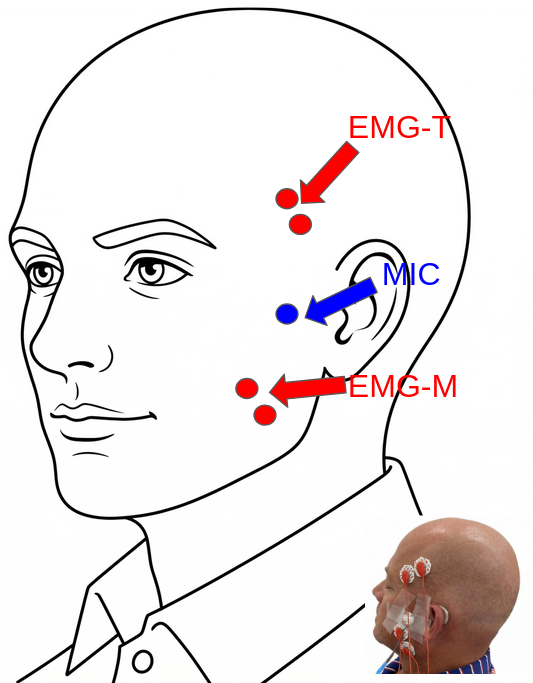
\includegraphics[width=0.9\linewidth]{Figures/patient_new.png}
  \caption{Sensor placement for data acquisition. Bipolar surface-EMG electrode pairs were positioned over the temporalis (EMG-T) and masseter (EMG-M) muscles. A microphone (MIC) was secured near the temporomandibular joint as an annotation aid; it is not analysed in this study, for the measured reasons given in Section~\ref{sec:mic}. This arrangement was evaluated only during instructed awake laboratory tasks.}
  \Description{A participant with surface-EMG electrodes over the jaw muscles and a microphone positioned near the temporomandibular joint.}
  \label{fig:sensor_setup}
\end{figure}

\subsection{The channel that is not analysed}
\label{sec:mic}

A single omnidirectional microphone was secured near the temporomandibular joint (Fig.~\ref{fig:sensor_setup}) and recorded alongside the electromyogram. Its intended role was to support offline annotation: an experimenter reviewing a trial can hear when tooth contact occurs, which is useful for confirming that a marked interval contains the instructed activity. It is not analysed here, and no result in this paper reads it.

It is excluded on measured grounds rather than on preference, and they are worth stating plainly so that the exclusion can be checked. First, the channel is not an acoustic waveform. It is integer-valued with a quantisation step of exactly 1 count over a range of roughly 50--227; 96\% of its power lies below 10~Hz (range 91.4--98.7\%), concentrated at the 1--3-Hz masticatory rhythm, so it behaves as a rectified sound-level output. At the 1200-Hz acquisition rate the 600-Hz Nyquist frequency also sits below the band in which tooth contact radiates most of its energy. Second, it is not synchronous with the electromyogram: over the 45 chewing recordings, where every muscle burst coincides with an impact, the envelope cross-correlation at zero lag has a median of $-0.017$ and peaks at a median absolute lag of 18~s. Third, and decisively, a rotation-invariant fingerprint of every channel of every recording shows 100 distinct waveforms on each of the four EMG channels but only 37 on the microphone channel: 83 of the 100 recordings carry a microphone waveform that is bit-identical, after a circular rotation, to another \emph{participant's} recording of the same condition. A leave-one-subject-out protocol therefore never holds that channel out, and no second copy exists to recover---the three surviving \texttt{.npy} acquisition companions reproduce the electromyographic and trigger columns exactly but contain an all-zero microphone column, and the video files carry no audio stream.

A matched modality ablation had in any case already been run on this channel before the fingerprinting audit, under the protocol described in Section~\ref{sec:training} and on the same windows, folds and seeds as everything else reported here. Adding the microphone branch to the EMG model changed participant-level macro-F1 by $+0.009$ on the five-class task and $+0.004$ with chewing removed, both smaller than the spread between training seeds; the microphone alone reached 42.8\% macro-F1 against 72.0\% for EMG alone. Those figures are consistent with a channel that contributes almost nothing, but they cannot be quoted as a measurement of what a microphone contributes, because of the duplication above. The defensible statement is the negative one: this channel was not usable, EMG carries the classification on its own, and the question of whether a working transducer would help is untested rather than answered. Section~\ref{sec:mic_discussion} states what a future collection would need to do differently.

The exclusion is enforced rather than remembered. The pipeline now computes a rotation-invariant fingerprint of every channel of every recording, groups them, and refuses any run whose held-out participant's signal appears in its own training set, at a cost of one pass over the data.

\subsection{Window labelling and analysable sample}

Every analysed window is required to lie \emph{wholly inside} one interval during which the trigger marks the participant as actively performing the named task, so that no window can span two conditions or a trigger transition. Windows are cut from the continuously filtered recording, never filtered individually, because filtering each window separately injects an edge transient exceeding one signal standard deviation into the first 50 samples of every example.

Three exclusions are applied before windowing, and each guard was measured rather than assumed. A \textbf{transition guard} of 0.25~s is removed on each side of every trigger edge: over 432 task onsets (358 with a detectable envelope transition) the median lag between the button press and the electromyographic onset was $-0.075$~s, muscle activity preceded the marker at 79.9\% of onsets, and among the 20\% of onsets in the harmful direction the median lag was 0.054~s and the largest ever measured was 0.352~s. A \textbf{startup guard} of 0.5~s is removed at the beginning of every recording, replacing an earlier unexplained 3-s skip; amplifier settling transients were observed in 66 of 100 recordings, all settled within 0.40~s, with peak excursions up to $12{,}580\times$ the recording's robust scale. Finally, quiet-rest windows are drawn only from the five dedicated rest recordings; trigger-off intervals inside active recordings are \emph{not} treated as rest, because they are unlabelled rather than verified as quiet. The rest class therefore represents quiet laboratory rest, not the full range of everyday non-event behaviour.

The recordings were consolidated into five experimental classes. \textbf{Rest} comprised windows from the five dedicated quiet-baseline recordings only. \textbf{Movement} included opening/closing, lateral deviation, and protrusion/retrusion. \textbf{Clenching} included molar clench, incisor clench, and unilateral left/right bite. \textbf{Grinding} included the instructed grinding trials. \textbf{Chewing} included cheese, carrots or popcorn, and gum. These categories contrast quiet non-event periods, non-chewing jaw movement, static loading, lateral tooth-contact activity, and functional mastication. Bracing and thrusting without tooth contact were not elicited and are not represented.

Chewing was included because it is a common functional activity and a plausible confound for an ambulatory jaw-activity classifier. Because it may also be comparatively easy to recognise, the primary five-class results are accompanied by a sensitivity analysis that excludes chewing, and by a second analysis that collapses the five labels into instructed clenching/grinding versus rest/movement/chewing.

Continuous signals were segmented into 1.0-second windows (1200 samples) with a 0.5-second stride (600 samples), creating 50\% overlap between adjacent windows. Under the containment and guard rules above, 100 recordings yielded 6,173 analysable windows from 99 recordings: 590 rest, 333 movement, 799 clenching, 816 instructed grinding, and 3,635 chewing (Table~\ref{tab:dataset}, Fig.~\ref{fig:sample_flow}). These counts supersede the 11,845 windows reported previously, which were produced by a legacy policy that labelled whole recordings rather than trigger-verified intervals and therefore included inter-trial and transition material inside activity classes. The two sets of counts are not comparable, and only the trigger-constrained counts are used here.

These windows are not independent observations: adjacent windows overlap by 50\%, many windows originate from the same recording, and all of them originate from only five participants. The participant, rather than the window, therefore defines the effective unit for generalisation, and all primary metrics below are computed within a participant before being summarised.

\begin{table}[h]
  \caption{Dataset characteristics under the trigger-constrained labelling policy.}
  \label{tab:dataset}
  \centering
  \small
  \begin{tabular*}{\columnwidth}{@{\extracolsep{\fill}}ll@{}}
    \toprule
    Property & Value \\
    \midrule
    Participants & 5 \\
    Recordings (contributing) & 100 (99) \\
    EMG channels analysed & 4 (2 bilateral pairs) \\
    Microphone channels analysed & 0 (recorded, excluded) \\
    Sampling rate & 1200 Hz \\
    Signal units & Arbitrary ADC units \\
    Window size & 1200 samples (1.0 s) \\
    Stride & 600 samples (0.5 s) \\
    Transition guard & 0.25 s each side \\
    Startup guard & 0.5 s per recording \\
    Rest windows & 590 \\
    Movement windows & 333 \\
    Clenching windows & 799 \\
    Grinding windows & 816 \\
    Chewing windows & 3,635 \\
    Total analysed windows & 6,173 \\
    Experimental classes & 5 \\
    Quiet-rest class & Included \\
    \bottomrule
  \end{tabular*}
\end{table}

\begin{figure*}[h]
  \centering
  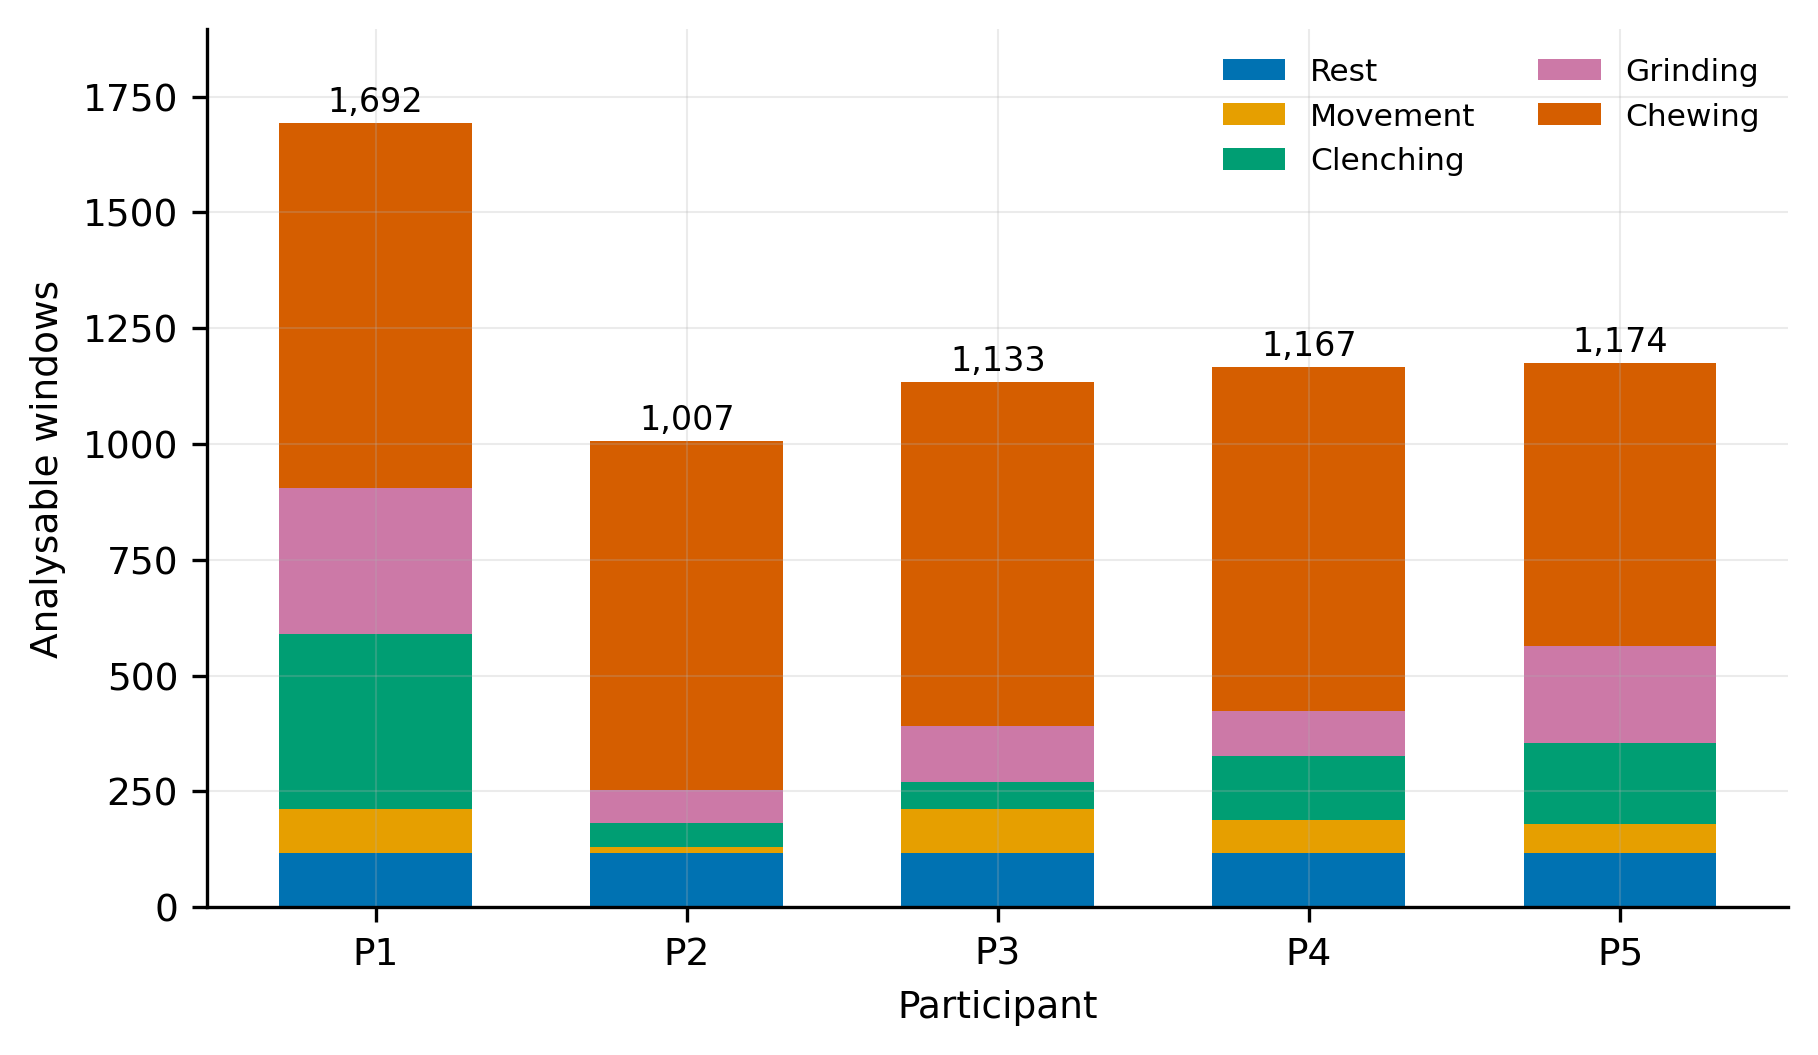
\includegraphics[width=0.78\linewidth]{Figures/v5/sample_flow.png}
  \caption{Analysable windows per participant and class after the containment, transition-guard and startup-guard exclusions. Participants are labelled P1--P5 here and in every later figure, in the same order as Table~\ref{tab:persubject}. Class sizes are strongly unequal both between classes---chewing supplies 58.9\% of all windows---and between participants within a class, which is why class weighting, minority-only augmentation and participant-level aggregation are all used. Section~\ref{sec:constraints} shows that the between-participant inequality is a consequence of how differently participants marked the trigger.}
  \Description{Stacked bar chart of window counts per participant, colored by task family.}
  \label{fig:sample_flow}
\end{figure*}

\subsection{Mains interference and the corrected filter chain}
\label{sec:filter}

Every result in this paper was regenerated after a spectral audit of the raw recordings. Because that audit is the subject of RQ1, its measurements are given here and its effect on classification is reported in Section~\ref{sec:rq1}.

The acquisition software applied its own fixed notch, recorded in every metadata sidecar, and that notch removed the 60-Hz fundamental before the data were written to disk. Interference survived at the harmonics instead. Measured against the local noise floor of the raw signals, the peaks at 180, 300, and 420~Hz ranged from tens of times that floor in the least affected participant to more than a million times it in the most affected. Across all 100 recordings, 62 had more than 30\% of their raw in-band EMG power concentrated within $\pm 3$~Hz of a mains multiple, and in the five dedicated quiet-rest recordings that share was 91.3--99.8\%.

The preprocessing chain used in earlier analyses of this dataset was a single 60-Hz notch ($Q=30$) followed by a 20--450-Hz band-pass. On the recordings described above it removed the only mains frequency that was already absent and passed every frequency that was present: the mains share of in-band power after filtering was 91.4--99.8\%, essentially unchanged from the raw signal (Fig.~\ref{fig:filter_fix}a, c). A filter-response plot of that chain looks entirely conventional, which is why the problem was not visible until the response was drawn over the measured spectrum of the data.

The corrected chain notches every mains multiple inside the pass band---60, 120, 180, 240, 300, 360, and 420~Hz---before the same fourth-order Butterworth band-pass from 20 to 450~Hz. Each notch is \emph{constant-width} (8~Hz at $-3$~dB, so $Q = f_0/8$) rather than constant-$Q$. Constant $Q$ would give a 2-Hz notch at 60~Hz and a 14-Hz notch at 420~Hz---that is, the narrowest response exactly where the hardware notch left a residue and the widest where nothing survives. Both variants remove 56~Hz of the 430-Hz pass band, an identical 13\% cost, but at that same cost the constant-width bank left the worst-contaminated cell at $3.2\times$ its local noise floor against $25.6\times$ for constant $Q$, an eight-fold reduction in residual interference. After correction, the mains share of in-band power in the quiet-rest recordings fell to 0.46--0.66\% (Fig.~\ref{fig:filter_fix}b, c). A comb filter and spectral interpolation were also implemented and measured on the same windows; both left more residual interference, and spectral interpolation is additionally acausal by construction.

The chain was selected on this interference criterion, which can be specified in advance, and not on held-out classification score. That distinction is not decorative here: the constant-$Q$ bank scored marginally \emph{higher} in screening classification (0.689 versus 0.679 macro-F1 on the same windows) while leaving eight times the residual interference, and choosing on score would have selected it. The measurable property was preferred to the score.

All filtering is zero-phase (forward--backward second-order sections), applied to the whole continuous recording before any window is cut. Zero-phase filtering reads samples from the future of each output sample. It is appropriate for the offline analysis reported here and it cannot support a streaming, wearable, or real-time claim; a causal mode exists in the implementation, and the mode used is recorded in every run bundle.

\begin{figure*}[t]
  \centering
  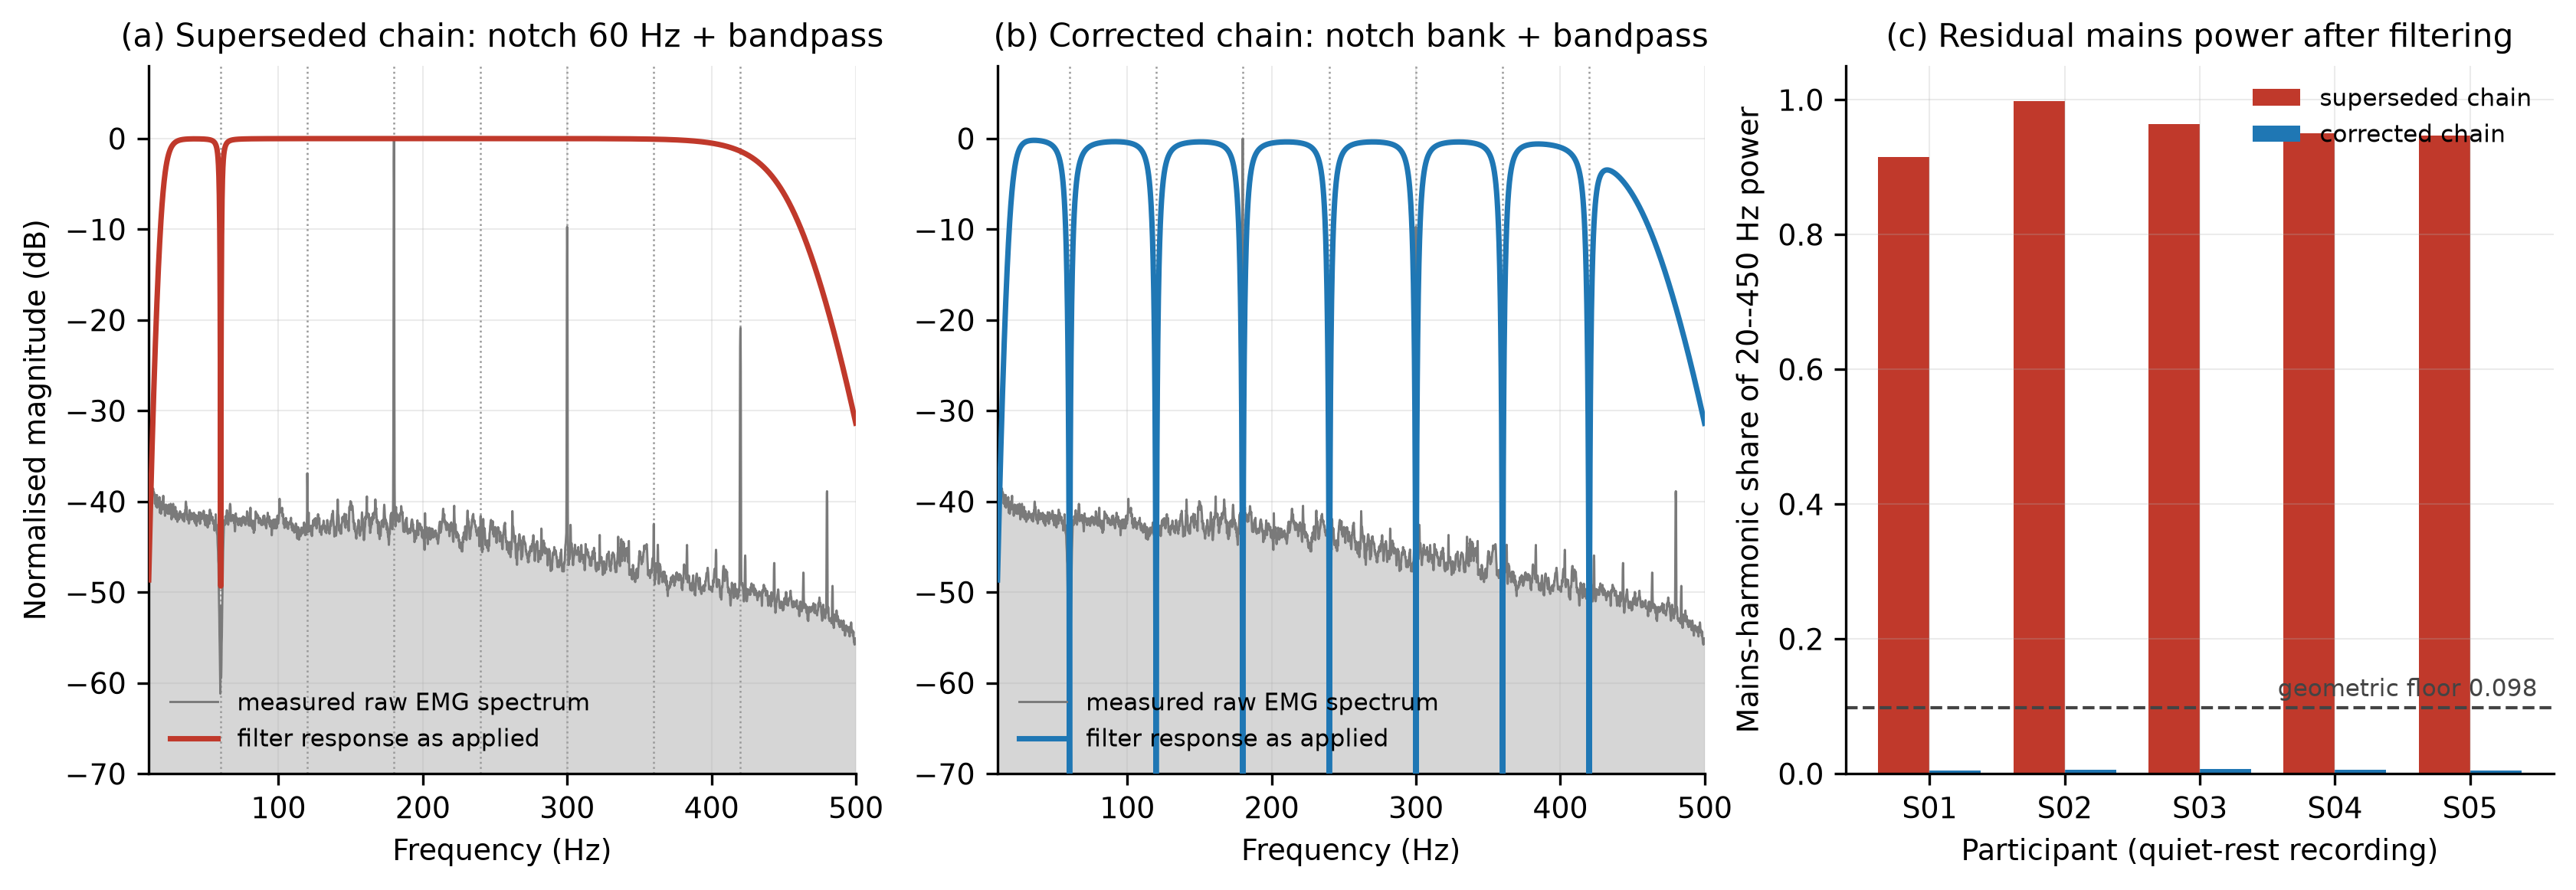
\includegraphics[width=\linewidth]{Figures/filter_defect_and_correction.png}
  \caption{The mains-harmonic defect and its correction. (a) The superseded chain: the 60-Hz notch lands where the acquisition hardware had already removed the fundamental, while the tall harmonic peaks at 180, 300 and 420~Hz pass through the band-pass untouched. (b) The corrected chain: seven constant-width notches land on the peaks. Gray traces are the mean raw EMG spectrum of the five dedicated quiet-rest recordings; colored traces are the zero-phase response as actually applied; dotted lines mark 60~Hz and its harmonics. (c) Share of 20--450-Hz power lying within $\pm3$~Hz of a mains multiple, per participant, after each chain. The dashed line marks the 0.098 share a perfectly white signal would score, because seven $\pm3$-Hz bands occupy 42~Hz of a 430-Hz pass band; a notch bank scores below it by deleting those bins.}
  \Description{Three panels: two filter responses drawn over the measured raw EMG spectrum, and a bar chart of residual mains power per participant.}
  \label{fig:filter_fix}
\end{figure*}

\subsection{Normalisation and wavelet decomposition}

EMG signals were z-scored per channel using means and standard deviations computed \emph{only} from the training participants of the fold in question. The list of participants that produced each fold's statistics is stored with the fold and asserted not to contain the held-out participant before that participant is evaluated. A per-participant (transductive) normalisation scope is implemented and prespecified as a separate configuration, and Section~\ref{sec:constraints} prices it, but it is not used for any confirmatory number reported here; the strict scope is the one that would support a deployment claim without a fitting session.

Figure~\ref{fig:emg_preprocessing} shows the chain on a real excerpt. Signals were then decomposed using the Daubechies-4 wavelet at four levels, and the sub-branches used $A_4$ ($<38$~Hz), $D_3$ (75--150~Hz), and $D_1$ (300--600~Hz, of which only the 300--450-Hz portion survives the band-pass). Daubechies wavelets were selected for their compact support and prior use in transient EMG analysis~\cite{englehart2003robust}. The pipeline now rejects any band that its own filter chain has removed, unless the configuration declares the exception explicitly.

\begin{figure*}[h]
  \centering
  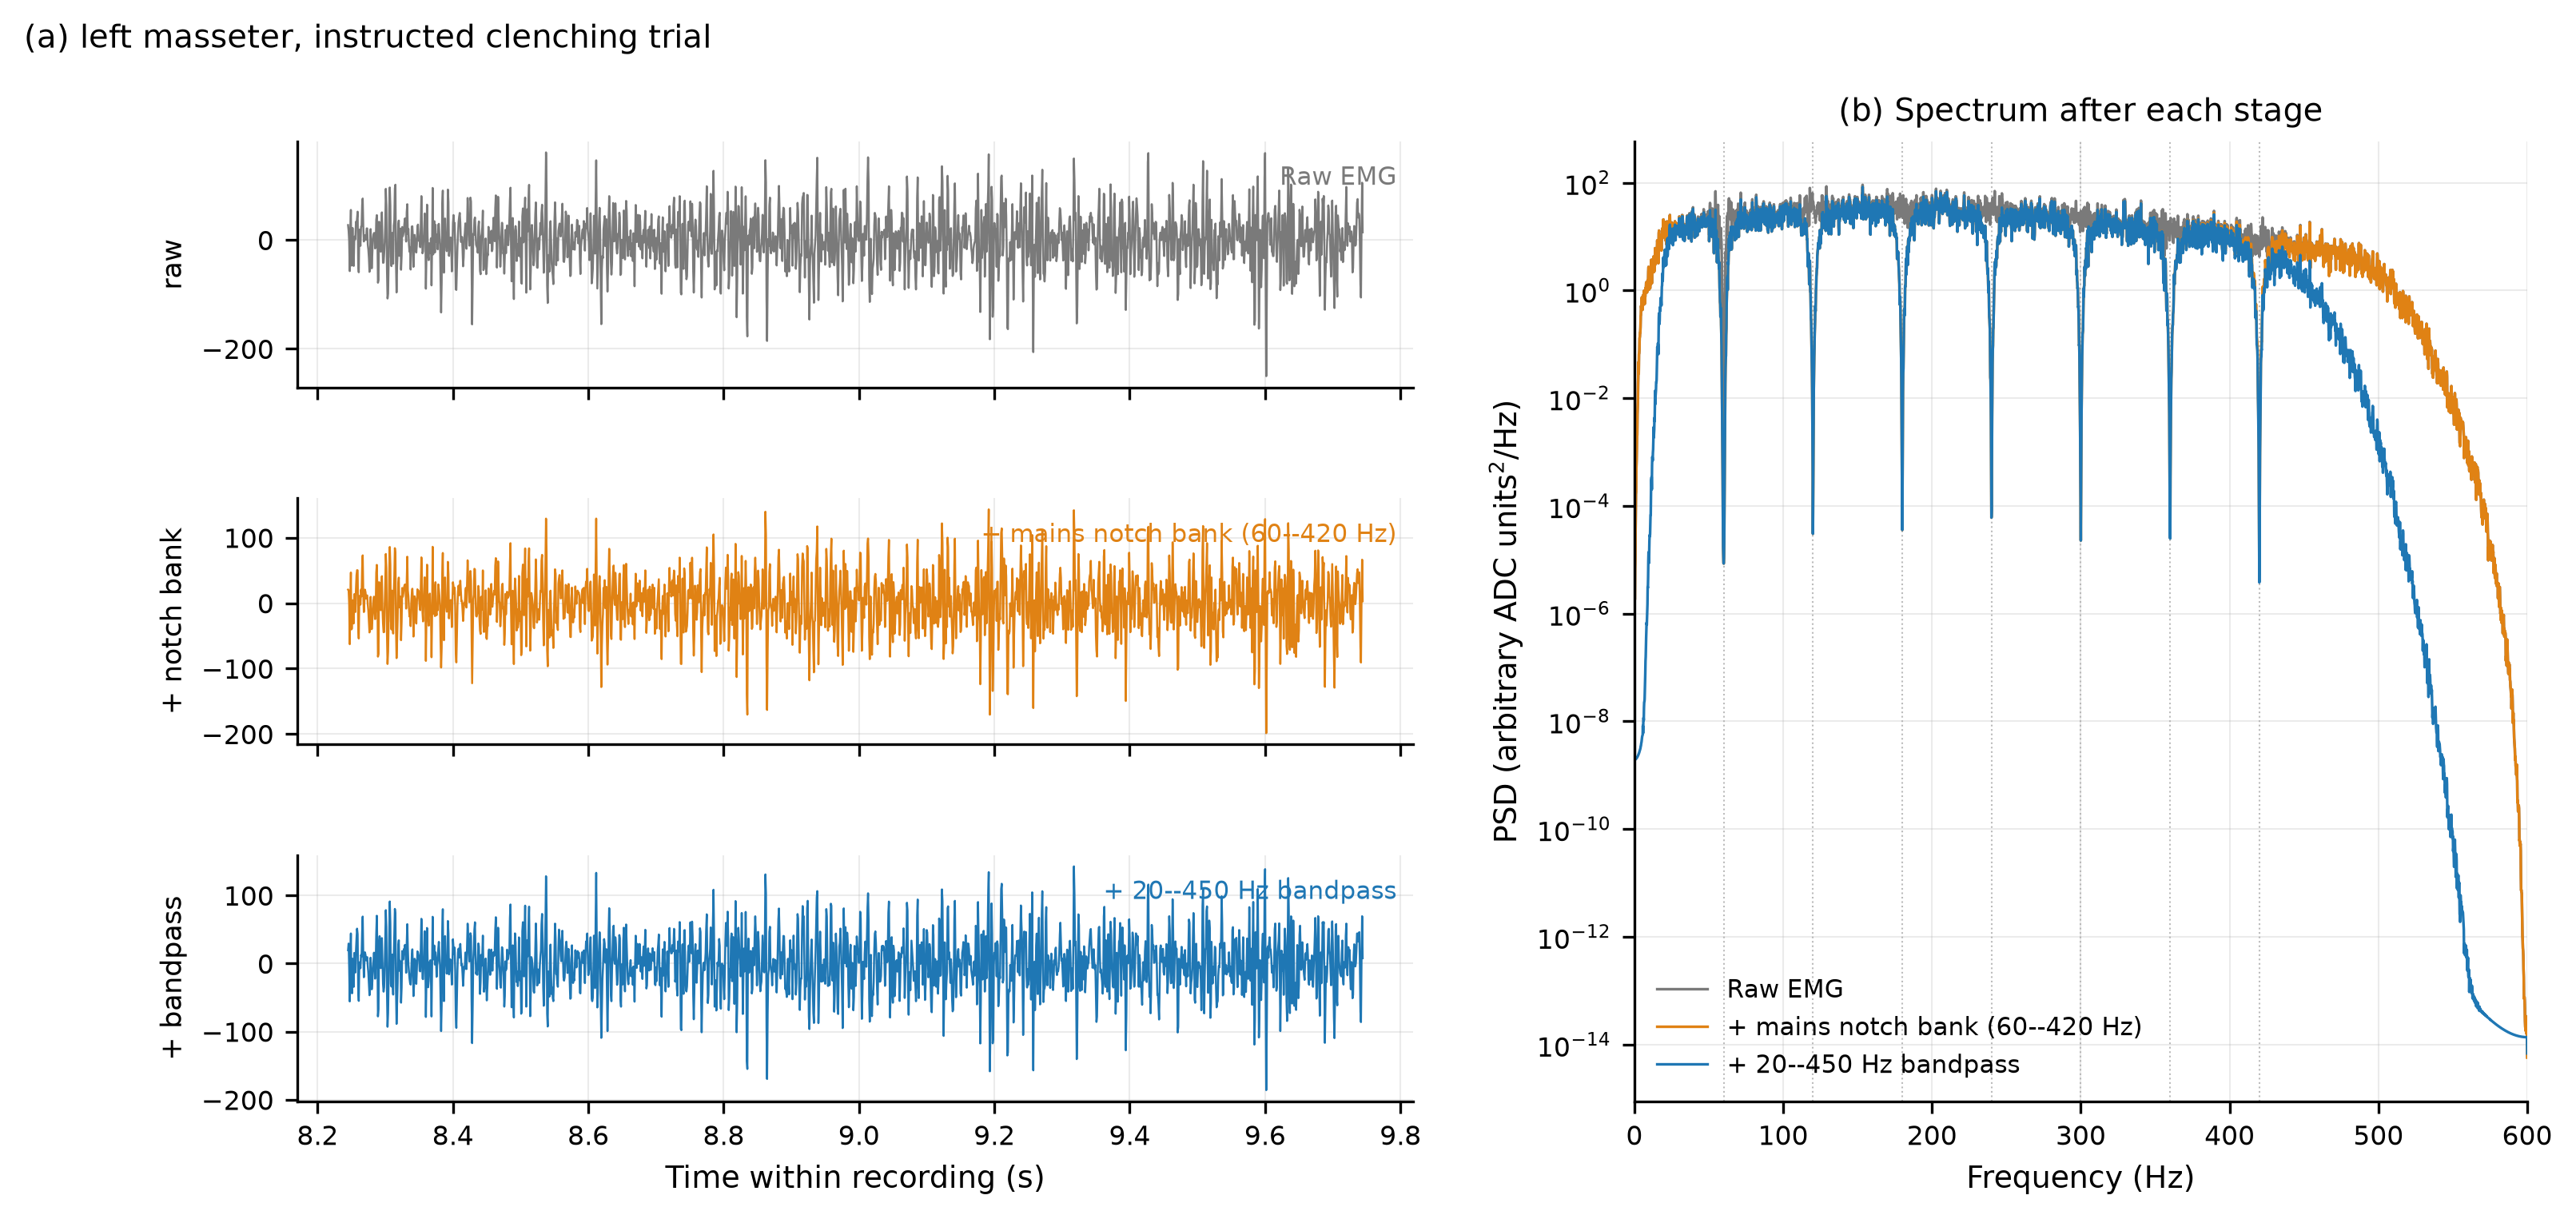
\includegraphics[width=\linewidth]{Figures/preprocessing_stages_5class.png}
  \caption{Production preprocessing on a real excerpt of an instructed clenching trial (left masseter channel). (a) Time domain after each stage. (b) Power spectrum after each stage; the notch bank removes the seven mains multiples marked by dotted lines and the band-pass then removes content outside 20--450~Hz. The chain is applied to the continuous recording and windows are cut afterwards.}
  \label{fig:emg_preprocessing}
\end{figure*}

\subsection{Model architecture}

The model is a single-branch wavelet convolutional network (Fig.~\ref{fig:architecture}). It contains three CNN sub-branches, one per retained wavelet band. Each sub-branch applies a 3-tap convolution to 8 channels, batch normalisation, a rectified linear unit, max pooling by 2, a second 3-tap convolution to 16 channels, batch normalisation, a rectified linear unit, and adaptive average pooling to a single value per channel, contributing 16 features per band and 48 features in total.

The 48 concatenated features are passed to a multilayer perceptron (MLP) with dimensions $48\rightarrow48\rightarrow32$. Batch normalisation, a rectified linear unit, and dropout with probability 0.5 are applied in each hidden layer. A final linear layer produces logits for rest, movement, clenching, grinding, and chewing. The complete model has 5,901 trainable parameters (1,656 in the wavelet branch, 4,080 in the MLP, and 165 in the classification head), or 23.1~KiB at 32-bit precision.

\begin{figure*}[t]
  \centering
  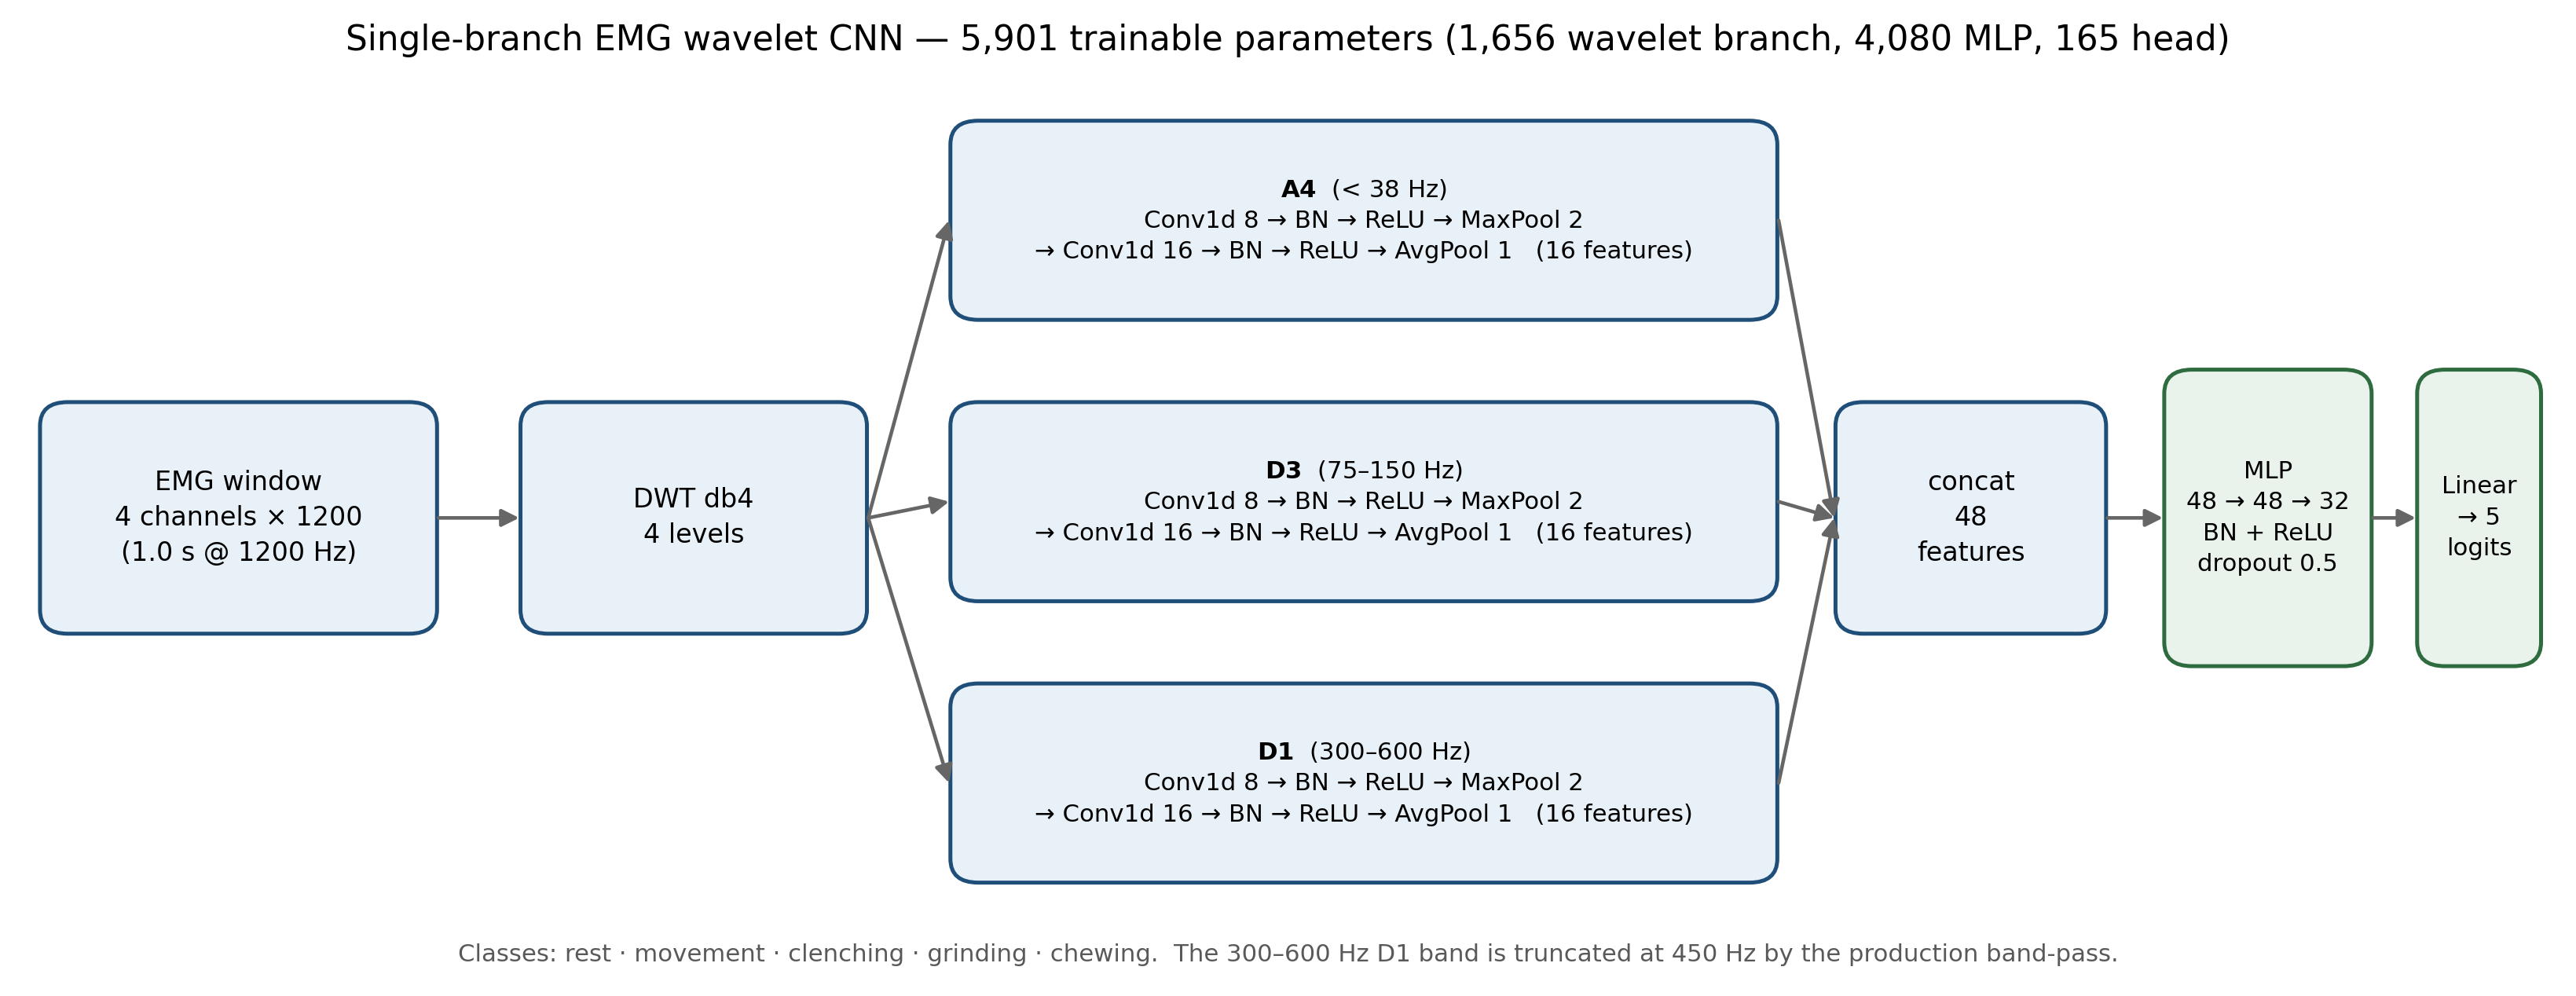
\includegraphics[width=\linewidth]{Figures/v5/architecture_emg.png}
  \caption{Single-branch wavelet CNN. The four EMG channels undergo a db4 decomposition; three retained bands are processed by parallel per-band CNN sub-branches, concatenated, and classified by an MLP with outputs for rest, movement, clenching, grinding, and chewing. Layer widths, wavelet family, band edges and parameter counts are read from the instantiated model rather than transcribed.}
  \Description{An EMG wavelet-CNN pathway with three per-band sub-branches feeding a five-output multilayer perceptron.}
  \label{fig:architecture}
\end{figure*}

\subsection{Training and evaluation}
\label{sec:training}

To address class imbalance after adding rest, the model used inverse-frequency class weights recomputed within each outer training fold, and augmentation of minority-class training windows by amplitude scaling in $[0.9, 1.1]$ (applied with probability 0.5), additive Gaussian noise at 2\% of the window standard deviation (probability 0.3), and circular shifts of up to $\pm50$ samples (probability 0.3). A window was eligible for augmentation with probability 0.4 and only if its class fell below 70\% of the largest class in that fold, so chewing windows were never augmented and rest windows were. Augmentation was applied only within the training partition of each fold, enforced structurally: the augmenter raises an error for any stage other than training, and each transformation is seeded by the triple (run seed, epoch, sample identifier) so that it does not depend on worker count or batch order.

Optimisation used AdamW with weight decay $1\times10^{-4}$, gradient clipping at norm 1.0, batch size 64, learning rate $1\times10^{-3}$, and focal loss~\cite{lin2017focal} with focusing parameter $\gamma = 1.5$. The loss and learning rate were fixed rather than searched, because this run was designed as a matched comparison across conditions and a fixed training configuration prevents any condition from winning by drawing a better hyperparameter. Table~\ref{tab:hyperparameters} lists the settings.

Evaluation used \emph{nested} leave-one-subject-out (LOSO). In each of the five outer folds, one participant was sealed as the test set and the remaining four entered a participant-grouped inner LOSO loop of four inner folds. Every normalisation statistic, class weight and augmentation minority set was fitted on inner-training participants only. The best epoch was recorded per inner fold by validation macro-F1, and the epoch budget for the final refit was the median of those best epochs. The model was then refit on all four outer-training participants for exactly that many epochs, with no early stopping and no validation set, and the held-out participant was evaluated exactly once. The held-out participant's sample identifiers are stored privately and released only by an explicit single-use call, so selection code cannot reach them even accidentally. Macro-F1 was the selection objective rather than accuracy, because accuracy is dominated by chewing. The whole protocol was run with three random seeds, all of which completed all five outer folds, and metrics are computed independently per seed and then summarised. Probabilities are never averaged across seeds and no seed is selected as best.

Across the fifteen fold--seed combinations the epoch budget ranged from 15 to 43 with a median of 19, and the five-class conditions took 1.1~h of the 4.8~h that the complete matched run required on the training hardware.

\textbf{Participant-level metrics are primary.} Accuracy, balanced accuracy, macro precision, recall, F1 and one-vs-rest ROC--AUC are computed within each held-out participant and then summarised across the five participants; all five individual values are reported. Pooled-window metrics are also reported, but only as descriptive summaries, because windows within a participant and recording are correlated. AUC was computed from the saved held-out class probabilities, never from hard labels or a confusion matrix. A class absent from a fold receives no AUC rather than an imputed value. No window-level bootstrap intervals or $p$-values are reported: the windows are clustered and overlapping, and with five participants such tests would overstate precision without supporting a population-level claim. Held-out probabilities are uncalibrated (expected calibration error 0.063); they must not be read as probabilities, but every AUC remains valid because AUC is rank-based and unaffected by any monotone rescaling.

Two secondary analyses were computed post hoc from the same held-out five-class predictions and are labelled as such. First, chewing windows were removed and the four remaining probabilities renormalised, giving a four-class problem over rest, movement, clenching, and grinding. Second, predictions and probabilities were collapsed into instructed clenching/grinding versus rest/movement/chewing. Both re-read one model rather than training a new one. A separately trained four-class model without chewing was also run, on the same windows and folds, as a check that the renormalisation is not doing the work. The second analysis provides a binary comparison against quiet rest and other instructed activities; it is task discrimination, not bruxism detection, because the positive tasks were elicited and the background class does not include unrestricted free-living behaviour.

\subsection{Feature baselines and the screening harness}
\label{sec:screening}

Two families of measurement in this paper come from a deliberately cheap \emph{screening} harness rather than from the confirmatory protocol above, and every value it produces is labelled as such wherever it appears. The harness extracts 28 hand-written features per window---per EMG channel, the log RMS of each of five db4 bands, the log waveform length, and the zero-crossing rate---and fits one model per outer fold with no nested hyperparameter selection. Two estimators are used: multinomial logistic regression and gradient boosting. Because the feature set was chosen after looking at these five participants and no nested selection is performed, screening numbers are directionally reliable and optimistic in level. They decide which change is worth a confirmatory run; they are never reported as a result.

The harness serves two purposes here. It supplies the matched before-and-after comparison for RQ1, in which the only thing that changes is the EMG filter chain (Section~\ref{sec:rq1}). And it supplies the hand-engineered baseline for RQ3 (Section~\ref{sec:rq3}), which is the relevant comparison for a network whose per-band sub-branches reduce each band to a pooled amplitude: if a learned representation cannot beat the band energies it is built from, the architecture is not earning its place. Both comparisons run on the identical 6,173 windows and the identical five outer folds as the confirmatory model.

\begin{table}[h]
  \caption{Training and evaluation configuration of the reported model. The loss and learning rate were fixed rather than searched, so that the modality and label-set conditions of the same run differ only in what they were asked to do.}
  \label{tab:hyperparameters}
  \centering
  \footnotesize
  \begin{tabular*}{\columnwidth}{@{\extracolsep{\fill}}ll@{}}
    \toprule
    Hyperparameter & Value \\
    \midrule
    Optimiser & AdamW \\
    Learning rate & $1\times10^{-3}$ \\
    Weight decay & $1\times10^{-4}$ \\
    Loss & Focal, $\gamma = 1.5$ \\
    Class weights & Inverse frequency, per fold \\
    Dropout & 0.5 \\
    Batch size & 64 \\
    Gradient clipping & Norm 1.0 \\
    Epoch budget & Median inner best (15--43, median 19) \\
    Seeds & 0, 1, 2 \\
    Outer / inner folds & 5 / 4, participant-grouped \\
    Normalisation scope & Strict (outer-training participants) \\
    \bottomrule
  \end{tabular*}
\end{table}

\section{Results}

The confirmatory results below come from the EMG conditions of one nested-LOSO run on the corrected signal (five outer folds $\times$ three seeds; 6,173 held-out window predictions per seed, 18,519 in total for the five-class task and a further 7,614 for the separately trained four-class task). Every value was recomputed from the saved prediction ledgers, in which each held-out window appears exactly once per task, model and seed. Screening values are marked wherever they appear.

\subsection{RQ1: what the measurement chain contributes}
\label{sec:rq1}

The filter chain was changed while the windows, folds and labels were held identical, so the comparison isolates the chain (Table~\ref{tab:filter}, Fig.~\ref{fig:measurement_chain}). Identical is meant literally: the 6,173 analysed windows, their five outer-fold assignments and their class labels are the same objects in both arms, verified by comparing the two prediction ledgers window by window.

The confirmatory network answers the question directly. Trained and evaluated under the same nested-LOSO protocol through the superseded chain, it reached 55.0\% accuracy, 43.5\% participant-level macro-F1 and a macro one-vs-rest AUC of 0.785. Through the corrected chain the matched condition reached 80.9\%, 72.8\% and 0.963---a gain of 29.3 points of macro-F1, 25.9 points of accuracy and 0.178 of AUC. The share of quiet-rest windows misread as clenching or grinding fell from 30.2\% to 6.1\% over the same change. The contrast is conservative rather than generous in two respects: the superseded run additionally searched the loss and learning rate inside each fold, where the corrected run fixed them, and both arms are the fused condition so that the two are like-for-like on modality, which gives the superseded arm an input channel it could exploit. The corrected EMG-only condition reported throughout the rest of this paper scores 72.0\% macro-F1, within a point of its fused counterpart.

The screening harness reproduces the effect with two much simpler estimators, which rules out an idiosyncrasy of the network. Through the superseded chain, logistic regression on the 28 EMG band-energy features reached 53.1\% accuracy and 37.3\% macro-F1; through the corrected notch bank, 78.3\% and 63.9\%---a gain of 26.5 points of macro-F1 and 25.2 points of accuracy. Gradient boosting moved from 38.8\% to 61.3\% macro-F1 over the same change. Three estimators of very different capacity therefore move by 22 to 29 points, and none of them saw a new window, a new label or a new fold.

The per-participant view shows how severe the earlier state was. Through the superseded chain, two of the five held-out participants were essentially unclassifiable: P1 scored 18.1\% macro-F1 at 26.9\% accuracy and P2 scored 5.4\% at 6.9\%, both at or below what a constant prediction would achieve, while P3--P5 scored 57.6--75.4\%. After the correction the same five participants span 61.4--82.4\%. A result that had looked like severe between-participant heterogeneity---the standard reading of such a spread, and the one that motivates transfer learning and per-user calibration---was substantially an artifact of interference that differed between recording sessions.

Three further measurements establish that the superseded chain was not merely suboptimal but inert, and explain the mechanism.

First, the 60-Hz notch was doing nothing at all. A control chain with \emph{no} mains removal whatsoever---band-pass only---scored 38.5\% macro-F1, within 1.2 points of the superseded chain's 37.3\% and comfortably inside the range of the two. Filtering the fundamental that the acquisition hardware had already removed was, to the precision this comparison can resolve, equivalent to not filtering at all.

Second, the interference was large enough to be the dominant signal. Expressed as each activity's median RMS divided by \emph{that participant's own} resting RMS---the contrast a classifier must exploit---the superseded chain left chewing at 1.6--7.2$\times$ rest and clenching at 1.6--5.2$\times$. After correction the same quantities are 8.5--35.7$\times$ and 8.1--27.0$\times$ (Fig.~\ref{fig:measurement_chain}c). The physiological contrast was present in the recordings the whole time; it was buried under interference that varied more between people than the physiology varied between conditions.

Third, that is exactly what the between-participant statistics show. The superseded chain left a $5.07\times$ spread between the largest and smallest participant median RMS, and 20 participant pairs in which one person's \emph{resting} EMG exceeded another person's \emph{active} EMG. After correction the spread is $2.97\times$ and there are no such pairs (Fig.~\ref{fig:measurement_chain}d). A model trained on the earlier signal could reduce its loss by learning which participant a window came from rather than what that participant was doing, and leave-one-subject-out is the protocol that then reports the consequence as poor generalisation. The screening arm shows the same per-participant pattern as the network (Fig.~\ref{fig:measurement_chain}b): P2, the participant who gained most, moved from 0.135---below the 0.165 a uniform guess would score---to 0.645.

\begin{table*}[t]
  \centering
  \caption{RQ1. The EMG filter chain is the only thing that varies: the same 6,173 windows, the same five outer-fold assignments and the same labels in every arm, verified window by window across the two prediction ledgers. Residual mains power is the share of 20--450-Hz power within $\pm3$~Hz of a mains multiple, averaged over participant $\times$ class cells; a perfectly white signal would score 0.098. ``Inv.'' counts participant pairs in which one person's resting EMG exceeded another person's active EMG. Differences quoted in the text are computed before rounding, so they may differ by 0.1 from the difference of the rounded values shown here.}
  \label{tab:filter}
  \footnotesize
  \begin{tabular*}{\textwidth}{@{\extracolsep{\fill}}lcccccc@{}}
    \toprule
    & \multicolumn{3}{c}{Measured signal properties} & \multicolumn{3}{c}{Participant-level macro F1} \\
    \cmidrule(lr){2-4}\cmidrule(lr){5-7}
    EMG chain & \shortstack{Residual\\mains} & \shortstack{Ampl.\\spread} & Inv. & \shortstack{Wavelet\\CNN$^{a}$} & \shortstack{Logistic\\reg.$^{b}$} & \shortstack{Grad.\\boost.$^{b}$} \\
    \midrule
    60 Hz notch only (superseded) & 0.673 & $5.07\times$ & 20 & 43.5\% & 37.3\% & 38.8\% \\
    Band-pass only (control) & 0.671 & $5.02\times$ & 20 & --- & 38.5\% & 39.2\% \\
    \midrule
    \textbf{Mains notch bank, 8 Hz (used)} & \textbf{0.012} & $\mathbf{2.97\times}$ & \textbf{0} & \textbf{72.8\%} & \textbf{63.9\%} & \textbf{61.3\%} \\
    \bottomrule
  \end{tabular*}
  \begin{flushleft}\footnotesize
  The notch bank was selected on residual mains power, a criterion specifiable in advance, not on classification score. A constant-$Q$ bank at the identical 13\% band cost scored marginally higher in screening (0.689 against 0.679 macro-F1 on the full 35-feature set) while leaving eight times the residual interference, and would have been selected by a score criterion.\\
  $^{a}$Confirmatory nested LOSO, three seeds, five outer folds. Both rows are the fused condition, so the two are like-for-like on modality; the superseded row additionally searched the loss and learning rate inside each fold, which the corrected row fixed, so the comparison favours the superseded arm on both counts. The corrected EMG-only condition reported elsewhere in this paper scores 72.0\%.\\
  $^{b}$Screening harness on the 28 EMG features: one fit per outer fold, no nested selection, feature set chosen after seeing these participants. Optimistic in level; reported here for the contrast and to show that it does not depend on model capacity.
  \end{flushleft}
\end{table*}

\begin{figure*}[t]
  \centering
  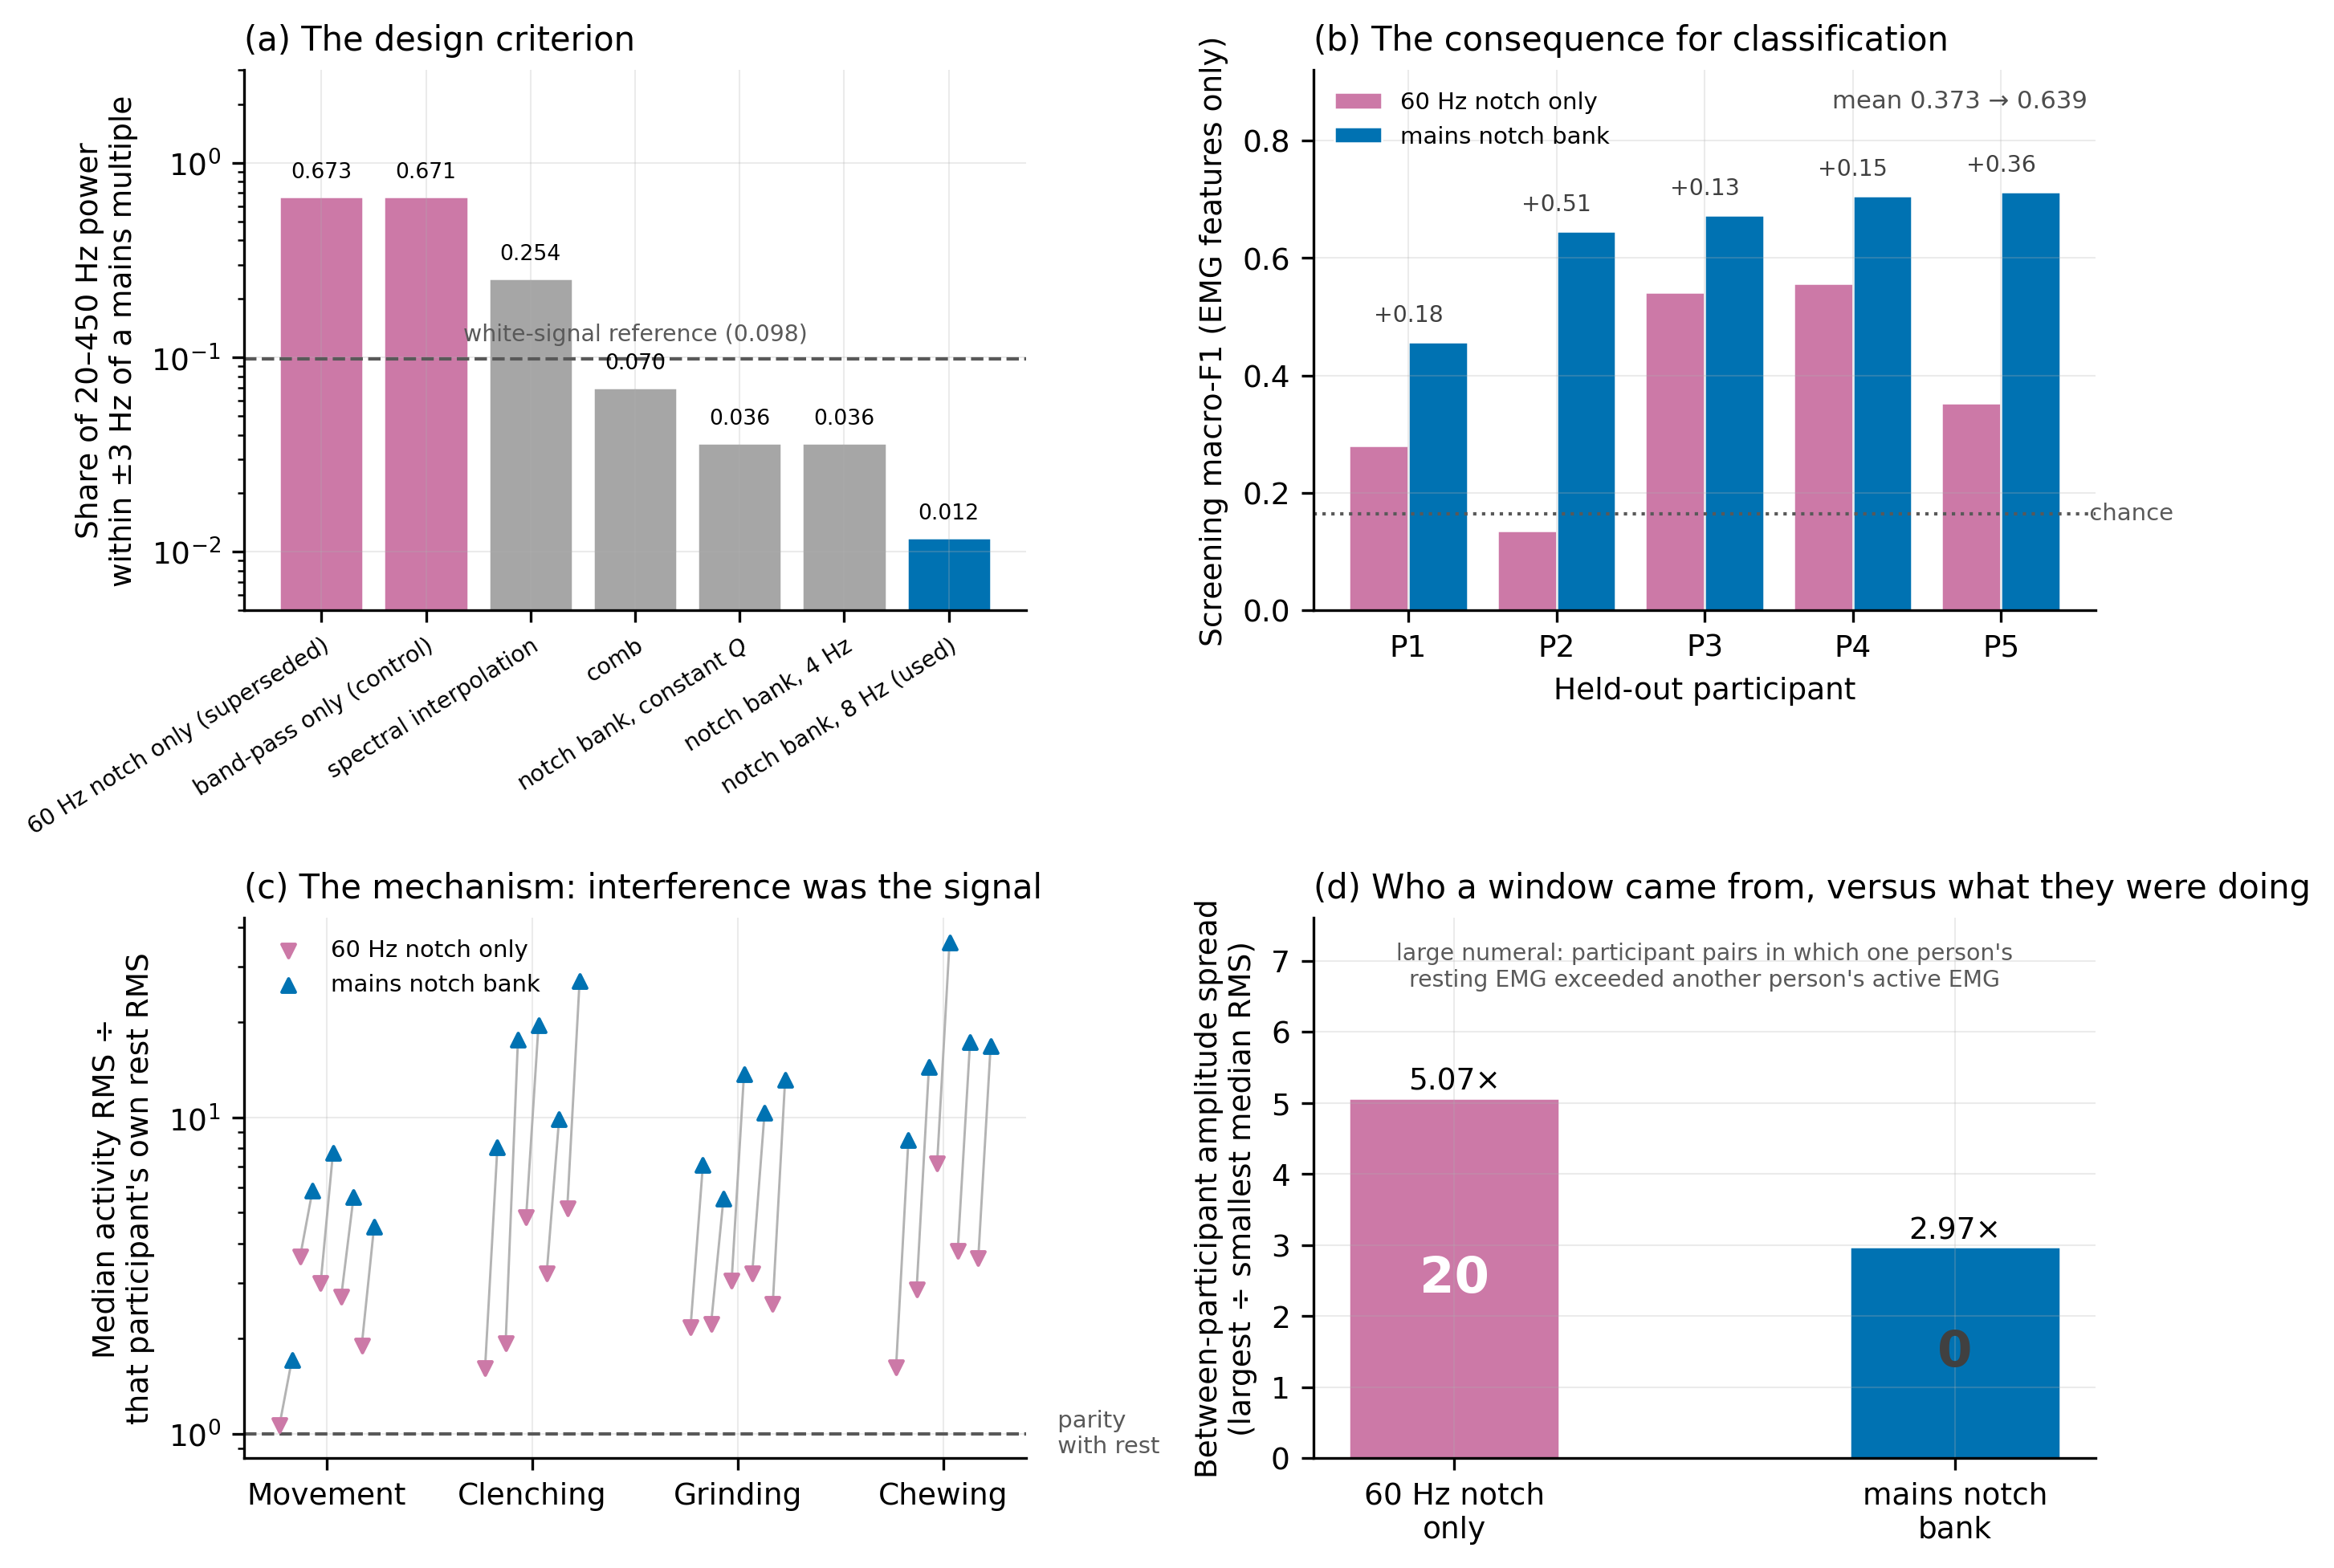
\includegraphics[width=\linewidth]{Figures/v5/measurement_chain.png}
  \caption{The mains-harmonic defect, expressed in the terms a classification paper is read in. (a) Residual mains power for every candidate chain that was implemented and measured, against the 0.098 a white signal would score; the chain used is the lowest, and was chosen on this axis rather than on classification score. (b) Screening macro-F1 per held-out participant before and after the correction, on the 28 EMG features and identical folds. (c) The mechanism: each activity's median RMS divided by that participant's own resting RMS, five participants per condition, before (down triangles) and after (up triangles). (d) Between-participant amplitude spread, and the number of participant pairs in which one person's resting EMG exceeded another person's active EMG. No panel of this figure reads the microphone.}
  \Description{Four panels showing residual interference by filter chain, per-participant classification gain, activity-to-rest amplitude contrast, and between-participant amplitude spread.}
  \label{fig:measurement_chain}
\end{figure*}

\subsection{RQ2: five-class performance on the corrected signal}

Averaged over the five held-out participants and three seeds, the model achieved 81.7\% accuracy, 77.6\% balanced accuracy, 72.0\% macro-F1, and a macro one-vs-rest ROC--AUC of 0.958 (Table~\ref{tab:results}). Seed-to-seed variation was small relative to the variation between participants: accuracy 83.4\%, 81.5\% and 80.2\%; macro-F1 74.5\%, 69.9\% and 71.4\%; macro AUC 0.963, 0.953 and 0.957. Pooling held-out windows across participants instead---a descriptive summary only, because the windows are correlated---gives 80.7\% accuracy, 69.4\% macro precision, 76.5\% macro recall, 71.5\% macro-F1 and a macro AUC of 0.948.

For the quiet-rest class the model achieved 77.1\% precision, 91.4\% recall, an F1 of 83.6\%, and a one-vs-rest AUC of 0.958 (Table~\ref{tab:perclass}). Rest is therefore the second-best-separated class after chewing and the best-recalled class of the five, which is the outcome the class was added to test: activity windows can be scored against a quiet non-event condition rather than only against one another.

Per-class one-vs-rest ROC and precision--recall curves are shown in Fig.~\ref{fig:roc_pr}. The ordering is consistent across both views, but the two views disagree sharply about how well the small classes are handled, and the disagreement is informative. For the seed drawn, movement combines an AUC of 0.949 with an average precision of 0.615, and instructed grinding an AUC of 0.921 with an average precision of 0.597; chewing, at 58.9\% prevalence, reaches 0.991 and 0.993. Precision--recall is sensitive to the very unequal class sizes and ROC is not, so a reader who sees only the AUC column of Table~\ref{tab:perclass} will overestimate how usable the minority classes are.

\begin{table*}[t]
  \centering
  \caption{Five-class performance on the corrected signal, averaged over the five held-out participants and three seeds. Classes are rest, movement, clenching, grinding, and chewing. The two baseline rows come from the screening harness of Section~\ref{sec:screening} on the identical windows and folds, and are optimistic in level, which makes the network's margin over them a conservative estimate. Values describe this five-participant dataset and are not population-level superiority tests.}
  \label{tab:results}
  \small
  \begin{tabular}{lccccc}
    \toprule
    Method & Accuracy & Macro prec. & Macro rec. & Macro F1 & Macro AUC \\
    \midrule
    \textbf{Wavelet CNN, 4-channel EMG} & \textbf{81.7\%} & \textbf{73.7\%} & \textbf{77.6\%} & \textbf{72.0\%} & \textbf{0.958} \\
    \midrule
    Logistic regression, band energies$^{a}$ & 78.3\% & -- & -- & 63.9\% & 0.965 \\
    Gradient boosting, band energies$^{a}$ & 74.8\% & -- & -- & 61.3\% & 0.914 \\
    \bottomrule
  \end{tabular}
  \begin{flushleft}\footnotesize
  Every value in this table is a participant-level mean, computed within each held-out participant and then averaged over the five, so the rows are directly comparable. The corresponding pooled-window macro AUCs are 0.948 for the CNN, 0.944 for logistic regression and 0.894 for gradient boosting.\\
  $^{a}$Screening harness: one model fit per outer fold, no nested hyperparameter selection, feature set chosen after seeing these participants. Optimistic in level. Macro precision and recall are not reported for these rows because the harness stores a prediction ledger rather than a per-class table.
  \end{flushleft}
\end{table*}

\begin{table*}[t]
  \centering
  \caption{Per-class performance on held-out windows, averaged over three seeds. AUC is one-vs-rest, computed from held-out probabilities.}
  \label{tab:perclass}
  \small
  \begin{tabular}{lccccc}
    \toprule
    Class & Precision & Recall & F1 & AUC & Windows \\
    \midrule
    Rest & 77.1\% & 91.4\% & 83.6\% & 0.958 & 590 \\
    Movement & 34.4\% & 69.8\% & 46.0\% & 0.937 & 333 \\
    Clenching & 70.5\% & 66.0\% & 68.1\% & 0.936 & 799 \\
    Grinding & 67.9\% & 69.5\% & 68.6\% & 0.928 & 816 \\
    Chewing & 97.3\% & 85.8\% & 91.1\% & 0.981 & 3,635 \\
    \midrule
    \textbf{Macro average} & 69.4\% & 76.5\% & 71.5\% & 0.948 & 6,173 \\
    \bottomrule
  \end{tabular}
\end{table*}

\begin{figure*}[h]
  \centering
  
\includegraphics[width=0.49\linewidth]{Figures/v5/five_class_roc_curves.png}
  \hfill
  
\includegraphics[width=0.49\linewidth]{Figures/v5/five_class_pr_curves.png}
  \caption{One-vs-rest ROC (left) and precision--recall (right) curves for the five experimental classes, pooled over the held-out windows of seed 0 (the lowest seed index, a fixed rule rather than a choice made after seeing the scores). Each curve depicts one trained model per fold, so the legend values are that seed's; the three-seed means are in Table~\ref{tab:perclass}. Precision--recall separates the classes far more sharply than ROC does, because it is sensitive to the very unequal class sizes.}
  \Description{Two panels of per-class ROC and precision-recall curves.}
  \label{fig:roc_pr}
\end{figure*}

\subsection{RQ3: learned representation against band energies}
\label{sec:rq3}

On the identical 6,173 windows and five outer folds, the screening harness reached 63.9\% macro-F1 at 78.3\% accuracy with logistic regression on 28 EMG band-energy features, and 61.3\% at 74.8\% with gradient boosting (Table~\ref{tab:results}). Every value is a participant-level mean computed exactly as the network's are, so the rows are comparable. The network's 72.0\% macro-F1 exceeds these by 8.1 and 10.6 points respectively, and its accuracy by 3.4 and 6.9. Because the screening harness fits one model per fold with a feature set chosen after seeing these participants, it is optimistic in level; the margin over it is therefore a conservative estimate rather than a generous one, and the direction is stable across two very different estimators.

The AUC column does not follow, and the discrepancy is worth stating rather than omitting. Logistic regression on band energies reaches a participant-level macro one-vs-rest AUC of 0.965 against the network's 0.958; on pooled held-out windows the ordering reverses, 0.944 against 0.948. Both differences are smaller than the network's own seed-to-seed AUC range (0.953--0.963), so the two models rank held-out windows about equally well and the network's advantage lies elsewhere: in where its decision boundaries fall once those windows are ranked. That is the same dissociation between ranking and thresholding that separates participants 1 and 4 below, and it is the reason macro-F1 rather than AUC was the prespecified selection objective.

Two further qualifications belong with this result, and both matter more than the margin.

The first is that this advantage was much smaller before the measurement chain was corrected. Through the superseded chain, on the identical windows and folds, the network reached 43.5\% macro-F1 against 39.3\% for logistic regression and 40.1\% for gradient boosting on the 35-feature screening set: a margin of 4.2 and 3.5 points, obtained by a network that additionally searched its loss and learning rate and additionally carried a microphone branch matched by seven of the baselines' features. That near-parity had been read at the time as evidence that the architecture was contributing nothing over band energies. The reading was correct about the numbers and wrong about the cause. When the dominant variance in a window is interference amplitude, a per-band pooled amplitude is all there is to extract, and a network whose sub-branches compute pooled band amplitudes cannot do better than features that compute them directly. Once the interference is removed the margin roughly doubles, to 8.1 and 10.6 points, against baselines that no longer read a second channel. The architecture's advantage is therefore a property of the corrected signal at least as much as of the architecture, and an architecture can be dismissed on the strength of a measurement defect.

The second is that this is a comparison against hand-engineered features, not against alternative learned architectures. A prespecified sweep of three deep baselines---a dual-branch temporal CNN that keeps the time axis, an early-fusion CNN on the raw signals, and a bidirectional LSTM---has not been rerun on the corrected signal, and the earlier measurements were taken through the defective chain and are superseded. RQ3 as answered here therefore establishes that the learned wavelet representation beats the band energies it is built from; it does not establish that this architecture is the best available one.

\subsection{Secondary analyses with rest}

When chewing was excluded, the remaining four-class problem comprised rest, movement, clenching, and grinding. Averaged over the held-out participants, this analysis yielded 77.7\% accuracy, 75.7\% macro-F1, and a macro AUC of 0.942; the corresponding pooled-window values were 75.4\% accuracy, 74.9\% macro precision, 76.1\% macro recall, 75.4\% macro-F1, and a macro AUC of 0.919 (Table~\ref{tab:sensitivity}). Removing chewing lowers accuracy by 4.0 percentage points but \emph{raises} macro-F1 by 3.7 points, because the metric is no longer dominated by a single large, easily separated class. A model trained separately on the same four classes reaches 77.7\% accuracy, 75.8\% macro-F1 and a macro AUC of 0.942---agreement to within a tenth of a point on macro-F1, which confirms that the post-hoc values are not an artifact of the renormalisation shortcut.

For a task-level binary analysis, clenching and grinding were treated as the positive group and rest, movement, and chewing as the comparison group. This yielded 92.5\% accuracy, 86.4\% precision, 84.8\% sensitivity, 95.3\% specificity, an F1 of 85.5\%, and a ROC--AUC of 0.970 on pooled windows, and 93.0\% accuracy with a participant-level macro-F1 of 89.3\% and AUC of 0.968. Within the quiet-rest condition, 7.7\% of rest windows (45, 50 and 42 of 590 across the three seeds) were classified as clenching or grinding. This analysis includes a laboratory non-event class but does not measure detection in a continuous free-living stream: a 7.7\% per-window false-alarm rate at a 0.5-s decision interval corresponds to roughly 550 false alarms per hour if the background were quiet rest throughout, which is the quantity a deployable detector must report and this design cannot estimate.

\begin{table*}[h]
  \caption{Secondary analyses computed post hoc from the held-out five-class predictions, averaged over three seeds. These re-read one trained model; they are not separately trained tasks.}
  \label{tab:sensitivity}
  \centering
  \begin{tabular}{lcccccc}
    \toprule
    Analysis & Accuracy & Precision & Recall & Specificity & F1 & AUC \\
    \midrule
    Excluding chewing$^{a}$ & 75.4\% & 74.9\% & 76.1\% & -- & 75.4\% & 0.919 \\
    Collapsed binary$^{b}$ & 92.5\% & 86.4\% & 84.8\% & 95.3\% & 85.5\% & 0.970 \\
    \bottomrule
  \end{tabular}
  \begin{flushleft}\footnotesize
  Values are pooled over held-out windows. The corresponding participant-level means are 77.7\% accuracy / 75.7\% macro-F1 / 0.942 AUC when chewing is excluded, and 93.0\% accuracy / 89.3\% macro-F1 / 0.968 AUC for the collapsed binary analysis.\\
  $^{a}$Macro precision, recall, F1, and one-vs-rest AUC across rest, movement, clenching, and grinding, after removing chewing windows and renormalising the remaining four probabilities. A separately trained four-class model on the same windows and folds reaches 77.7\% accuracy and 75.8\% participant-level macro-F1.\\
  $^{b}$Instructed clenching/grinding treated as positive; rest/movement/chewing treated as the comparison group. This is task discrimination, not clinical diagnosis.
  \end{flushleft}
\end{table*}

\subsection{Class-level diagnostics}

The highest per-class F1 was observed for chewing (91.1\%) and the lowest for movement (46.0\%). Movement's low F1 is a precision problem rather than a detection problem: its recall is 69.8\% and its one-vs-rest AUC is 0.937, but its precision is 34.4\% because it is the smallest class (333 windows, 5.4\% of the total) and absorbs 9.9\% of the 3,635 chewing windows, which are eleven times more numerous. Clenching and grinding are the hardest pair to separate: 19.5\% of clenching windows were labelled grinding and 14.5\% of grinding windows were labelled clenching, which together account for the majority of both classes' errors. Rest had the highest recall of any class at 91.4\%, and its dominant error was into grinding (7.5\%, against 0.3\% into clenching), so confusion between quiet rest and the combined instructed clenching/grinding group occurred in 7.7\% of rest windows. These errors carry the most weight, because they approximate false alarms under the limited quiet-rest condition.

The held-out confusion matrix is shown in Fig.~\ref{fig:confusion}. For the seed shown, the diagonal counts were 534 of 590 rest windows, 242 of 333 movement, 542 of 799 clenching, 589 of 816 grinding, and 3,187 of 3,635 chewing.

We used t-distributed stochastic neighbour embedding (t-SNE)~\cite{vandermaaten2008visualizing} to visualise the 32-dimensional penultimate representation of held-out windows (Fig.~\ref{fig:tsne}). Chewing occupies several large, well-separated regions, consistent with its high AUC and with food-dependent rhythmic structure. Rest forms a small number of tight, compact islands, which is what a low-variance quiet condition should look like. Clenching and instructed grinding share adjacent and partly interleaved territory rather than separate ones, and movement windows appear mostly as a scatter along the borders of the larger classes. The embedding therefore reproduces the two error patterns visible in the confusion matrix. t-SNE distances are not metric, so the embedding is used only as corroboration and no quantitative claim rests on it.

\begin{figure*}[h]
  \centering
  
\includegraphics[width=0.72\linewidth]{Figures/v5/tsne_5class.png}
  \caption{t-SNE visualisation of the 32-dimensional learned penultimate representation for held-out windows, coloured by experimental class. Chewing occupies large separate regions and rest forms tight compact islands, whereas clenching and instructed grinding interleave and movement scatters along class borders. Embeddings were recomputed from the saved fold checkpoints using only outer-test windows of one seed, so each held-out window appears exactly once.}
  \Description{Two-dimensional scatter plot of held-out windows colored by the five experimental classes.}
  \label{fig:tsne}
\end{figure*}

\begin{figure*}[h]
  \centering
  
\includegraphics[width=\linewidth]{Figures/v5/confmatrx_5class.png}
  \caption{Held-out confusion matrix for rest, movement, clenching, grinding, and chewing, pooled across the five leave-one-subject-out folds of seed 0 (selected by the fixed lowest-seed-index rule, not by score). (a) Counts. (b) Row-normalised recall. The two dominant error patterns are the mutual clenching--grinding confusion and the leakage of chewing windows into the much smaller movement class.}
  \Description{A five-by-five confusion matrix shown as counts and as row-normalized recall.}
  \label{fig:confusion}
\end{figure*}

\subsection{Participant-level results}

Table~\ref{tab:persubject} reports five-class results for each held-out participant. Across participants, accuracy ranged from 73.4\% to 90.7\%, macro-F1 from 63.2\% to 80.5\%, and macro AUC from 0.904 to 0.981 (Fig.~\ref{fig:per_participant}). The spread is substantial relative to the mean and is not explained by class balance alone.

Two participants illustrate why accuracy and AUC should be read together. Participant 4 had the lowest accuracy alongside the second-highest macro AUC (74.0\% and 0.981): its held-out windows are ranked well by the model's scores, and the loss is concentrated in where the decision boundaries fall for that participant rather than in the model's ability to order its windows. Participant 1 shows the opposite pattern---the lowest AUC (0.904) and the lowest macro-F1 (63.2\%), at an accuracy no better than participant 4's---and it also contributes the largest single share of windows (1,692 of 6,173), so it dominates any pooled-window summary while counting as one of five in the participant-level summary. This is one concrete reason the participant-level aggregation is treated as primary here.

These five values describe internal LOSO behaviour. With five participants the tabulated standard deviations describe the sample rather than a sampling distribution, and no population-level estimate follows from the mean.

\begin{table}[h]
  \caption{Five-class performance for each held-out participant, averaged over three seeds.}
  \label{tab:persubject}
  \centering
  \footnotesize
  \begin{tabular*}{\columnwidth}{@{\extracolsep{\fill}}lrrrr@{}}
    \toprule
    Held out & $n$ & Acc. & Macro F1 & Macro AUC \\
    \midrule
    Participant 1 & 1,692 & 73.4\% & 63.2\% & 0.904 \\
    Participant 2 & 1,007 & 90.7\% & 72.6\% & 0.957 \\
    Participant 3 & 1,133 & 83.7\% & 71.3\% & 0.967 \\
    Participant 4 & 1,167 & 74.0\% & 72.2\% & 0.981 \\
    Participant 5 & 1,174 & 86.7\% & 80.5\% & 0.980 \\
    \midrule
    Mean & 6,173 & 81.7\% & 72.0\% & 0.958 \\
    SD & --- & 7.7 & 6.1 & 0.032 \\
    \bottomrule
  \end{tabular*}
\end{table}

\begin{figure*}[h]
  \centering
  
\includegraphics[width=0.72\linewidth]{Figures/v5/five_class_per_participant.png}
  \caption{Macro-F1 for each held-out participant. Each bar is the mean over the three seeds of that participant's own leave-one-subject-out fold, the open markers are the three individual seeds, and the label inside each bar gives that participant's held-out window count. Five participants cannot characterise population variability, so no generalisation claim follows from the mean.}
  \Description{Bar chart of per-participant macro F1 with the mean marked.}
  \label{fig:per_participant}
\end{figure*}

\subsection{Three design constraints larger than the architecture}
\label{sec:constraints}

RQ1 showed that one element of the measurement chain outweighed every modelling choice. Three further elements of the experimental and analysis design can be priced from the same archive, and two of them are worth more than the 8.1-point architectural margin of Section~\ref{sec:rq3}. All three are screening measurements, on the identical windows and folds, and are reported for direction and magnitude rather than as results.

\textbf{The one-second window is a binding constraint, not a tuned parameter.} Chewing and grinding are distinguished from clenching partly by \emph{rhythm}: burst--relaxation cycles at roughly 1--2~Hz, visible in Fig.~\ref{fig:signal_comparison}c, which a 1.0-s window can barely contain. Averaging held-out probabilities over consecutive windows raises screening macro-F1 monotonically from 0.730 at 1.0~s of context to 0.744 at 1.5~s, 0.769 at 2.5~s, 0.787 at 3.5~s and 0.804 at 5.5~s, before flattening at 0.799 by 8.5~s (Fig.~\ref{fig:design}a). A gain of 7.4 points from context alone is comparable to the gain from the architecture and larger than any other modelling change we evaluated. It must be read strictly as a \emph{trial-level} secondary analysis: every recording here contains a single condition, so averaging within a recording approaches a majority vote over a homogeneous trial. It is valid evidence that one second is too short and invalid as continuous-stream detection.

\textbf{The window/guard rule interacts with how participants used the trigger.} Participants marked trigger intervals at very different granularity---67 runs of median 8.7~s for P1 against 167 runs of median 1.7~s for P2---and a 1.0-s window with a 0.25-s guard on each side requires a run longer than 1.5~s to emit even one window. The consequence is severe and uneven: P1's clenching trials, marked as 14 long runs of median 9.0~s, emit 376 windows, while P2's, marked as 59 runs of median 1.7~s, emit 53, and P2's movement trials emit 11. Holding the window at 1.0~s and sweeping only the guard from 0 to 0.5~s moves the total from 6,779 to 5,610 windows but moves the smallest participant $\times$ class cell from 50 to 1; shortening the window to 0.5~s with a 0.1-s guard yields 13,983 windows and a smallest cell of 128 (Fig.~\ref{fig:design}b). The reported policy is a deliberate compromise between this pressure and the previous one, which pull in opposite directions. The real resolution is to stop forcing a fixed window onto variable-length trigger runs, and to standardise trigger use at collection time.

\textbf{Normalisation scope is worth about as much as the architecture.} Under the strict scope used for every confirmatory number here---statistics from outer-training participants only---the screening classifier reaches 0.639 macro-F1. Standardising each participant's features by that participant's own unlabelled distribution raises it to 0.730, a gain of 9.1 points, slightly more than the network's margin over the same features (Fig.~\ref{fig:design}c). This is transductive test-time adaptation, not label leakage: it reads the held-out participant's feature distribution but never their labels. It is nevertheless excluded from every reported result, because it would require a per-user fitting session and therefore describes a different product than a model that works out of the box. A robust (median/IQR) variant of the same scope gains only 0.9 points, and normalising per recording destroys the task entirely (0.036 macro-F1), because each recording contains one condition and per-recording standardisation removes precisely the between-condition amplitude difference the task depends on.

\begin{figure*}[t]
  \centering
  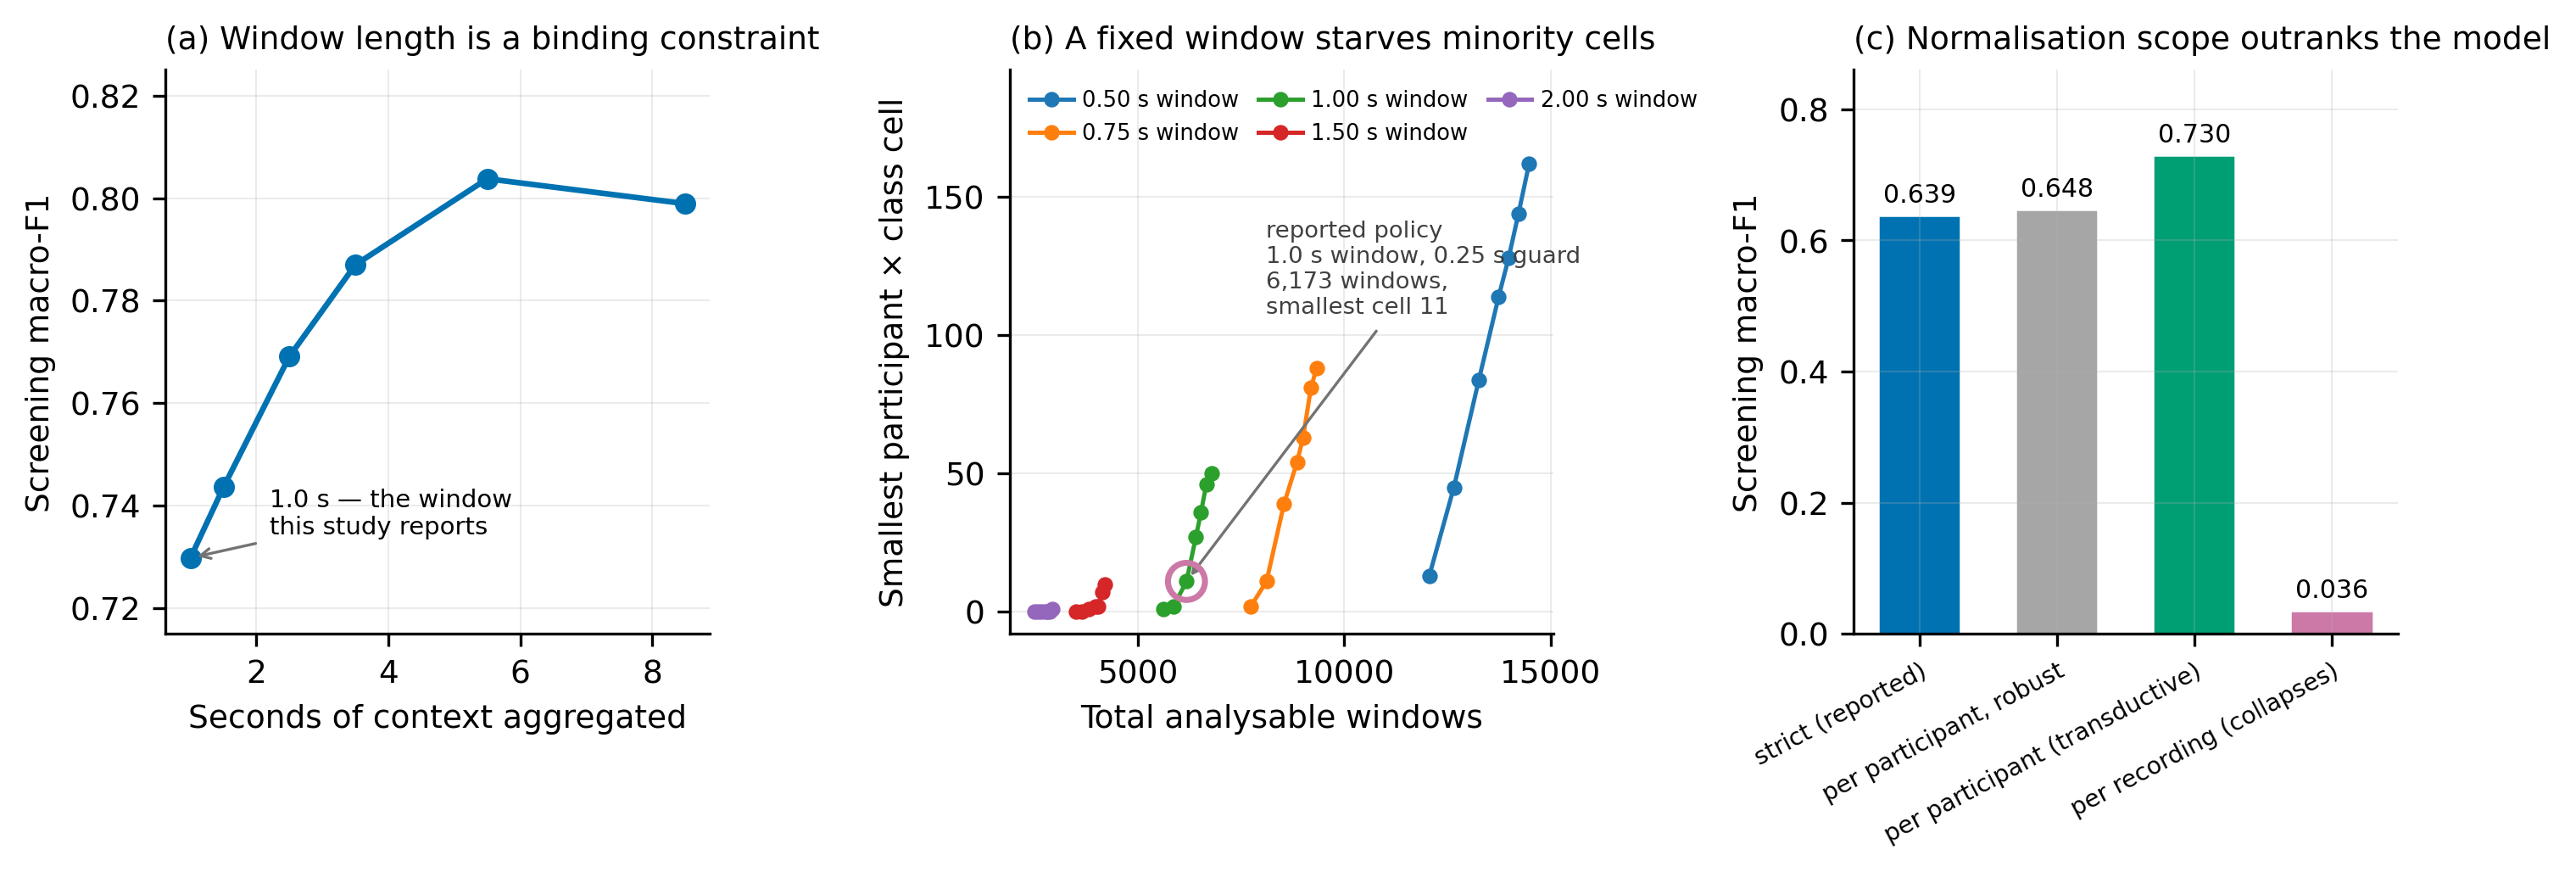
\includegraphics[width=\linewidth]{Figures/v5/design_constraints.png}
  \caption{Three design constraints, all measured on the identical windows and folds with the screening harness and the 28 EMG features. (a) Screening macro-F1 against seconds of temporal context aggregated within a recording; monotone across the whole range, so the 1.0-s window is a constraint rather than a tuned parameter. TRIAL-LEVEL: each recording holds one condition, so this is a labelled secondary analysis and not stream detection. (b) Every window/guard setting the audit swept: total analysable windows against the smallest participant $\times$ class cell, with the reported policy circled. The curves separate by window length because trigger granularity differed sharply between participants---67 runs of median 8.7~s for P1, 167 of median 1.7~s for P2, 132 of 2.9~s for P3, 141 of 2.9~s for P4 and 116 of 3.9~s for P5---so the same rule emits very different counts from each. (c) Feature normalisation scope. The transductive per-participant scope is worth more than the architecture, and is used by no reported number.}
  \Description{Three panels: macro-F1 versus temporal context, window count versus smallest class cell, and macro-F1 by normalisation scope.}
  \label{fig:design}
\end{figure*}

\subsection{Training behaviour and computational measurements}

Because the final model of each fold is refit for a fixed epoch budget chosen inside that fold, there is no early stopping and no validation set at refit time; the curves in Fig.~\ref{fig:loss_curves} are training-fit diagnostics, and the held-out participant appears in none of them. Budgets ranged from 15 to 43 epochs (median 19) across the fifteen fold--seed combinations, and training loss had largely flattened by the end of each budget. The gap between the final training-fit macro-F1 and the corresponding held-out macro-F1 averaged 0.144 and ranged from $-0.027$ to 0.291; per participant the mean gap was 0.276 for P1, 0.153 for P3, 0.129 for P4, 0.120 for P2 and 0.040 for P5. The ordering tracks the per-participant held-out scores of Table~\ref{tab:persubject} almost exactly---the largest gap belongs to the participant whose windows are the most numerous and the least well ranked---which is the expected signature of between-participant variation rather than of optimisation failure.

\begin{figure*}[h]
  \centering
  
\includegraphics[width=0.92\linewidth]{Figures/v5/training_curves_5class.png}
  \caption{Refit training loss (a) and training-fit macro-F1 (b) for all fifteen fold--seed combinations, coloured by held-out participant. Line style encodes the seed: solid seed 0, dashed seed 1, dotted seed 2. Each refit runs for the epoch budget chosen inside its own fold, so the curves end at different epochs. The held-out participant contributes to no curve and is scored once, after training ends.}
  \label{fig:loss_curves}
\end{figure*}

The model contains 5,901 trainable parameters and occupies 23.1~KiB at 32-bit precision. Three latencies must be kept separate. The \emph{input-context latency} is 1000~ms: the window length, and therefore the earliest point at which any decision about an event can exist. The \emph{decision update interval} is 500~ms, the stride. The \emph{processing latency}---the forward pass for one pre-segmented window at batch size 1 on an Intel CPU---has a median of 0.95~ms and a 95th percentile of 0.97~ms, giving an earliest possible decision at about 1001~ms. For reference on the same bench, an early-fusion CNN (19,141 parameters) took 0.20~ms and a bidirectional LSTM (10,309 parameters) 1.30~ms.

Compute time alone is not detection latency, and none of these measurements supports a wearable or real-time claim. No streaming implementation exists, the production filter chain is zero-phase and therefore acausal, and the measurements were taken on laptop and desktop hardware. Power consumption, end-to-end latency, wireless synchronisation, and reliability on a wearable device remain unmeasured.

\section{Discussion}

\subsection{What this study establishes}

Two findings survive scrutiny, and they are of different kinds.

The measurement finding is the larger one. On these recordings, whether the mains harmonics were removed determined more about what a classifier could learn than the architecture, the loss function, the feature set, or the estimator---29.3 points of macro-F1 for the confirmatory network, and 22 to 27 for two much simpler classifiers, against 8.1 for the architecture, all on the same windows, folds and labels. It is worth being precise about why this is not merely a story about one bad filter. The defect was not a coding error, and no amount of testing would have caught it: the code implemented exactly the filter it was asked for, the filter was the one the literature recommends, and its response plot is textbook-correct in isolation. What was missing was a single comparison---the filter response drawn over the measured spectrum of the actual recordings---and a single statistic, the share of in-band power sitting within a few hertz of each mains multiple. Both cost one pass over the data. Neither appears in the studies this work is compared against, so a reader has no way to tell whether a published accuracy in this area describes physiology or interference.

The way the defect presented is worth as much attention as its size. It did not look like a signal problem. It looked like between-participant heterogeneity---two of five held-out participants near chance, three in the normal range, a spread of 70 points of macro-F1---which is the most familiar failure mode in this literature and the one that motivates transfer learning, per-user calibration and larger cohorts. All three would have been reasonable responses, and none would have worked. A defect in a shared measurement chain expresses itself as apparent variation between the people measured through it, because interference amplitude varies with electrode impedance, cable routing and session rather than with physiology, and leave-one-subject-out then attributes that variation to the person held out.

The classification finding is narrower and conditional on the first. On the corrected signal, four channels of surface EMG and 5,901 parameters separate five instructed experimental conditions at a participant-level macro-F1 of 72.0\% and a macro one-vs-rest AUC of 0.958, under a protocol in which no held-out participant's windows touched normalisation, class weighting, augmentation, or training. Quiet rest---the class added to test whether activity can be scored against a non-event condition rather than only against other activities---proved the most reliably recovered class of the five, at 91.4\% recall and an AUC of 0.958. The residual 7.7\% of rest windows assigned to clenching or grinding is the most decision-relevant number in the paper, because it is the closest available analogue of a false alarm.

The architectural claim is real but bounded, and its most interesting property is that it is contingent. A learned wavelet representation beats the band energies it is built from by 8.1 points of macro-F1---though not on AUC, where a linear model on those same band energies ranks held-out windows equally well, so what the network buys is better placed decision boundaries rather than better ordering. And through the defective chain even the macro-F1 comparison was a tie, and was read at the time as evidence that the architecture was superfluous. Both readings were arithmetically correct. When interference amplitude dominates the variance of a window, there is nothing in a band but its amplitude, and an architecture that pools each band to an amplitude has no advantage over features that compute one directly. Architectural comparisons are therefore conditional on signal quality in a way that is rarely stated, and an architecture can be dismissed on the strength of a measurement defect.

\subsection{What the design constraints imply for a next study}

Section~\ref{sec:constraints} priced three choices that this design fixed early, and two of them turned out to be worth more than the architecture. That ordering is the practical message of the paper for anyone planning a follow-on collection.

Temporal context is the clearest. Performance rises monotonically from 1.0 to 5.5~s of context and the gain is 7.4 points, so the 1-second window is a limitation of this analysis rather than an optimum it found. A next-stage design should either classify variable-length segments directly or aggregate over a declared context, and must then evaluate on continuously varying activity rather than single-condition trials, because the aggregation measured here is a majority vote over a homogeneous trial and cannot be presented as event detection.

Trigger granularity is the least obvious and the easiest to fix. Because participants were free to mark bouts as they saw fit, one participant produced seven times as many clenching windows as another from the same instructed task, and the smallest participant $\times$ class cell in the analysed set holds 11 windows. That is not a modelling problem; it is an instruction problem, and it would be removed at source by standardising how the trigger is used, by recording continuous condition intervals rather than participant-marked bouts, or by both.

Normalisation scope is a product decision disguised as a preprocessing one. Standardising by the held-out participant's own unlabelled distribution is worth 9.1 points, uses no labels, and is entirely legitimate---but it presumes a per-user fitting session and therefore describes a device the user calibrates rather than one that works immediately. We report the strict scope throughout because it is the one that supports the weaker and more defensible claim, and we report the gap so that a future design can decide deliberately rather than by default.

\subsection{Why the microphone was excluded, and what would make it answerable}
\label{sec:mic_discussion}

The microphone recorded alongside the electromyogram is not analysed, and Section~\ref{sec:mic} gives the measurements behind that decision. Two points deserve emphasis in the context of the rest of this paper, because they are the same point twice.

The first is that the defect is invisible from any single recording. Every affected file is individually well-formed, correctly sized, and carries plausible values; the duplication is apparent only when two files are compared. A data audit that examines recordings one at a time therefore cannot detect it, which is precisely why our own first audit---thorough, reproducible, and pointed at the electromyogram---did not reach it. The check that does detect it is cheap and modality-agnostic: a rotation-invariant fingerprint of every channel of every recording, grouped, with a refusal if any held-out participant's signal appears in its own training set.

The second is that this determines what may be said next. An underpowered result and an invalid input are different problems with different remedies: more participants would address the first, and only a new acquisition addresses the second. We therefore do not report a weak fusion benefit, and we do not report that a microphone does not help. The honest position is that the question is untested. Answering it would require a documented transducer with a stated frequency response and output type, a sampling rate matched to the band in which tooth contact actually radiates, verified time alignment against the electromyogram, and a per-recording channel-integrity check run before any model is fitted. Figure~\ref{fig:signal_comparison} shows what the electromyogram alone contains for the three conditions in question; whether a working acoustic channel would add to it is a matter for a future collection.

\begin{figure*}[t]
  \centering
  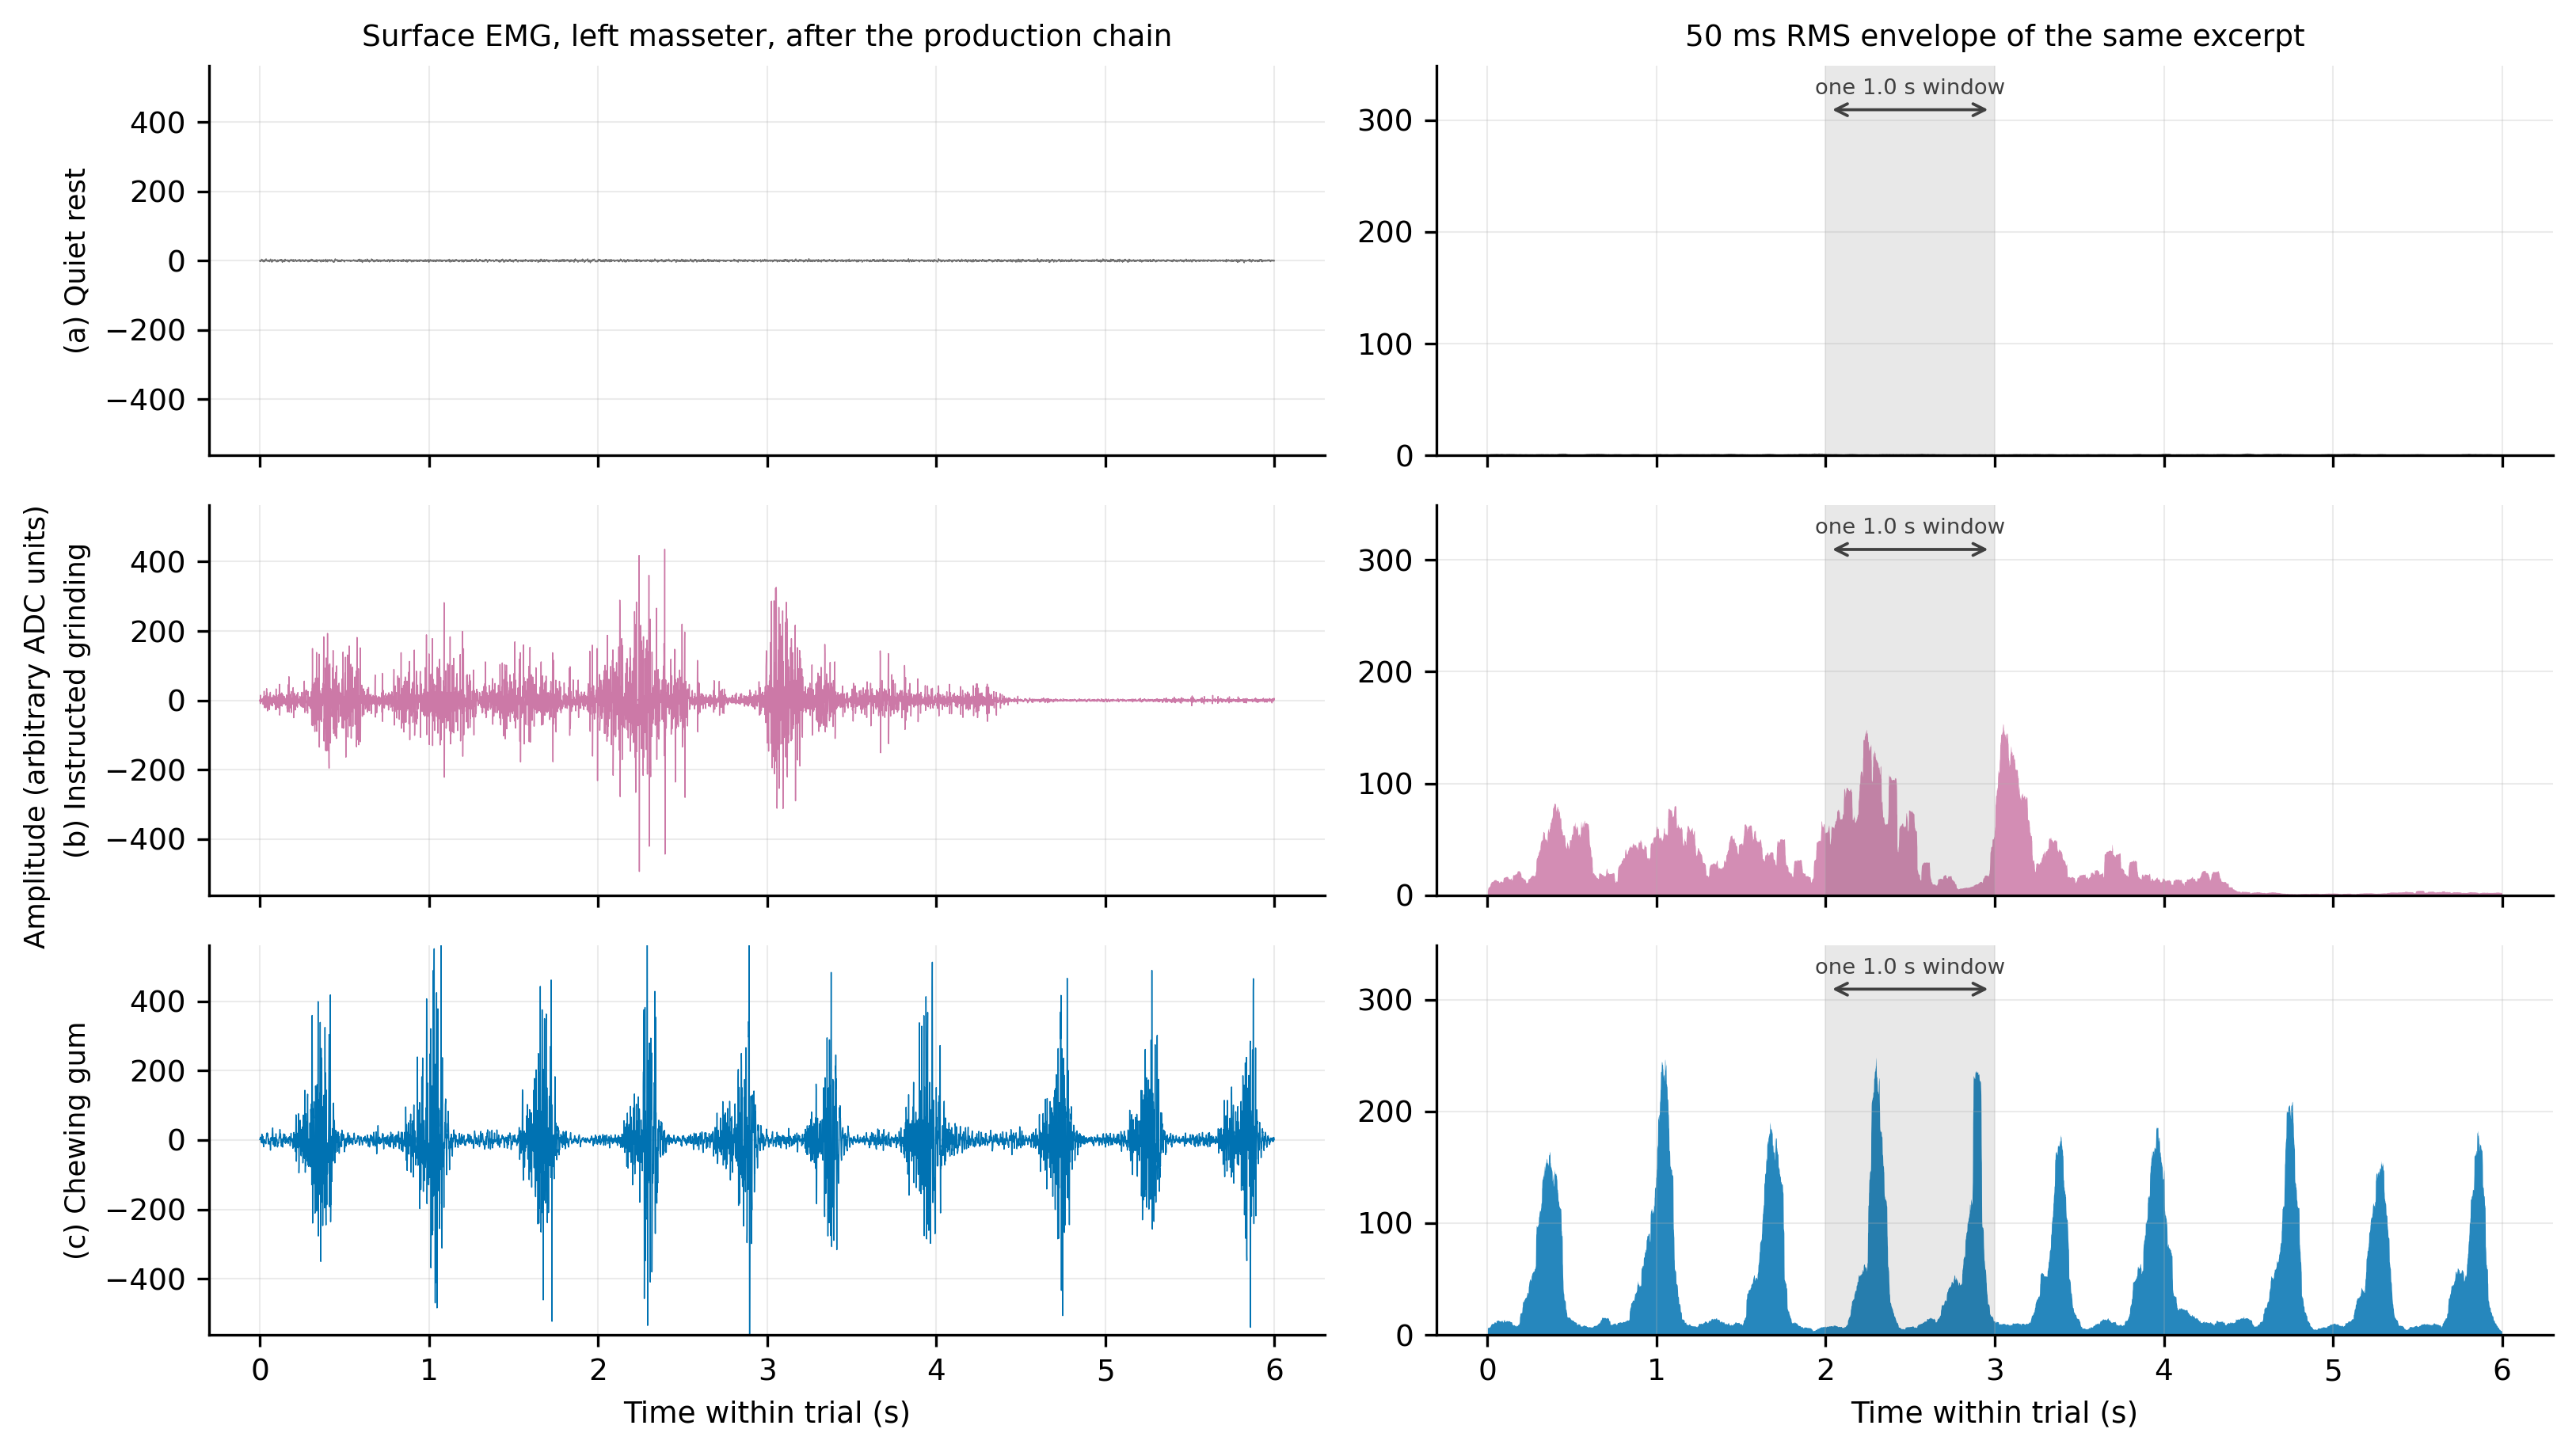
\includegraphics[width=\linewidth]{Figures/v5/signal_comparison_emg.png}
  \caption{Six-second excerpts of one participant's quiet rest, instructed grinding, and gum chewing after the corrected production chain, on a common scale, with the 50~ms RMS envelope of the same excerpt beside each. (a) Rest is quiet. (b) Instructed grinding produces sustained activation without a clear burst--relaxation rhythm. (c) Chewing produces rhythmic bursts separated by relaxation intervals at roughly 1.4~Hz. The shaded interval in the right column is one 1.0-second analysis window drawn to scale: it contains barely one chewing cycle, which is the constraint quantified in Fig.~\ref{fig:design}a.}
  \Description{Three rows of EMG traces and their envelopes for rest, instructed grinding and chewing, with a one-second window marked.}
  \label{fig:signal_comparison}
\end{figure*}

\subsection{Effect of the chewing class}

Chewing was selected as a relevant functional confound. In the five-class model it comprised 58.9\% of the windows and achieved an F1 score of 91.1\%, the highest of any class. Excluding it changed participant-level accuracy from 81.7\% to 77.7\% and macro-F1 from 72.0\% to 75.7\%. The direction of those two changes is the point: a headline accuracy computed over this class distribution is carried substantially by the easiest and largest class, whereas macro-F1 improves once that class is removed because the remaining four are more evenly sized. Reporting both analyses, and macro-F1 alongside accuracy throughout, is what prevents the largest class from carrying the summary.

The clenching--grinding split was retained because the two tasks differ in what a sensor sees. Clenching is static isometric loading, grinding is lateral excursion under load, and a system intended to characterise tooth-contact activity should be tested on whether it resolves them rather than credited for collapsing them. It is the hardest distinction in the five-class problem---19.5\% of clenching windows were labelled grinding and 14.5\% of grinding windows the reverse---and a 1-second window drawn from a grinding bout that passes through a static phase may legitimately carry either label, so part of the confusion is task-label ambiguity rather than model error. The collapsed analysis, in which the distinction is not required, reaches 92.5\% accuracy and an AUC of 0.970. Reporting both is what makes the cost of the distinction visible.

Comparison with the greater-than-90\% accuracy reported by Sonmezocak and Kurt using EMG alone~\cite{sonmezocak2021detection} is not like-for-like. Their classes included jaw opening, clenching, rhythmic grinding, and fatigue/pain; the present classes include rest, movement, clenching, grinding, and chewing. Dataset composition, preprocessing, sample size, and validation design also differ, and our evaluation is leave-one-subject-out, so every reported number is measured on a participant the model has never seen. A within-participant or window-shuffled split of the same data would score considerably higher without measuring anything about a new user. The two studies answer different classification questions, and the numerical accuracies do not establish that either method is superior.

\subsection{Toward continuous and home recording}

Laboratory repetitions do not capture the frequency, duration, or day-to-day variability of behaviour outside the laboratory. Multi-day, 24-hour home EMG recording has been shown to be feasible and illustrates its own difficulties~\cite{colonna2023electromyographic}. A next-stage awake study should combine multi-day EMG with a clearly defined background class and blinded annotation of candidate episodes, and should report day-level and participant-level performance including false positives per hour. It should also, on the evidence of Section~\ref{sec:constraints}, classify segments rather than fixed one-second windows, and standardise trigger or annotation granularity at collection time.

No conclusion about sleep follows from these awake laboratory tasks. A sleep study would require overnight data, appropriate sleep staging and event criteria, comparison with a suitable reference such as polysomnography or validated portable assessment, and repeated nights to evaluate night-to-night variability~\cite{cidverdejo2024instrumental}. Separate models may be required for awake and sleep contexts.

\subsection{Validity and limitations}

The principal limitation is the cohort size ($N=5$). The 6,173 overlapping five-class windows provide many optimisation examples but do not replace independent participants: adjacent windows share half their samples, and a single participant contributed 27\% of them. Window-level confidence intervals or tests would overstate precision and are deliberately not reported, and LOSO does not establish external generalisation when only five people are available. The between-participant spread observed here---accuracy from 73.4\% to 90.7\% and macro-F1 from 63.2\% to 80.5\%---is itself the clearest evidence that a five-person mean is not a population estimate. Age, facial anatomy, subcutaneous tissue, dentition, electrode placement, skin impedance, behaviour intensity, and prior diagnosis may all affect the EMG signal.

The architecture comparison is partial, and its scope is stated rather than implied. RQ3 establishes that the learned wavelet representation beats hand-engineered band energies from the same bands, on identical windows and folds and against an optimistic baseline. It does not establish that this architecture beats other learned architectures: the prespecified sweep of a temporal CNN, an early-fusion CNN and a bidirectional LSTM has not been rerun on the corrected signal, and the pre-correction measurements are superseded rather than reproducible. Given the finding of Section~\ref{sec:rq3}---that the architectural ranking inverted when the signal changed---rerunning that sweep on the corrected signal is the single most informative outstanding experiment.

The RQ1 contrast is measured on one cohort of five participants recorded in one laboratory, and its magnitude should not be read as a general effect size for mains correction. What generalises is the mechanism and the check, not the 29.3 points. Two features of the comparison are worth restating because they bound it in opposite directions: both arms of the confirmatory contrast are the fused condition, so the superseded arm carried an extra input channel and additionally searched its loss and learning rate, which makes the gap conservative; but the two runs also differ in the version of the codebase that produced them, and although the window set, fold assignment and labels are byte-identical and were verified as such, we cannot exclude that some unrecorded difference contributes. The screening arms, which share a single code path across both chains, move by a similar amount and are the cleaner evidence on that specific point.

Several analysis choices remain declared but unexercised. Held-out probabilities are uncalibrated (expected calibration error 0.063); temperature scaling is implemented but was not applied, so the scores must not be read as probabilities, though every reported AUC is unaffected. The per-participant normalisation scope and the temporal aggregation of Section~\ref{sec:constraints} are both implemented and both excluded from every reported result, for the reasons given there.

Task coverage and label precision bound what the classes mean. The task set covers tooth-contact clenching and grinding but not bracing or thrusting without tooth contact, and the participants' prior diagnoses were not phenotyped for this study. Class membership rests on a button press confirmed by the experimenter, and the alignment audit showed that muscle activity preceded the marker at four of every five onsets, with a median lag of $-0.075$~s; the 0.25-s transition guard exceeds the median error in the harmful direction and covers the 95th percentile, but 7\% of trial-leading windows may still carry a partially mislabelled edge. The acquisition token for the grinding condition was a filename label chosen at recording time, and the corresponding class is reported throughout as instructed grinding. Because every activity was performed on instruction, the recorded activity may be more regular, longer, or more forceful than spontaneous activity---a bias in the optimistic direction---and no spontaneous episode was verified against a reference standard.

Including quiet rest removes one limitation of an activity-only design, but the background data remain incomplete. Rest was recorded in a controlled laboratory and did not systematically sample speaking, swallowing, facial expression, head movement, coughing, eating outside the scripted task, environmental noise, or other free-living behaviours. The five-class analysis can estimate confusion against quiet rest---7.7\% of rest windows fell into the clenching/grinding group---but it cannot estimate false alarms per hour during unrestricted use, because the denominator that matters there is unrestricted behaviour and this design does not contain any.

Finally, the reported computational measurements were obtained on laptop and desktop hardware rather than a wearable prototype, and the acausal filter chain means they do not describe a streaming system.

\section{Conclusion}

This five-participant proof-of-concept study asked what a compact wavelet convolutional network can do with four channels of surface EMG, and found first that the answer depends more on the measurement chain than on the network. A spectral audit showed that the acquisition hardware had already removed the 60-Hz mains fundamental and that the surviving interference was harmonic, carrying 91.3--99.8\% of the in-band power of the quiet-rest recordings; the conventional chain removed the one frequency that was absent and passed everything that was present, and was indistinguishable in effect from applying no mains filter at all. Replacing it with a constant-width harmonic notch bank moved the matched nested-LOSO network from 43.5\% to 72.8\% participant-level macro-F1 on byte-identical windows, folds and labels, and two much simpler classifiers by 22 to 27 points over the same change; quiet-rest false alarms fell from 30.2\% to 6.1\%, the between-participant amplitude spread from $5.07\times$ to $2.97\times$, and all 20 participant pairs in which one person's resting EMG had exceeded another person's active EMG disappeared. Two participants who had scored 5.4\% and 18.1\% macro-F1 moved into the range of the other three.

On the corrected signal, and under leakage-free nested leave-one-subject-out evaluation, the model achieved a participant-level accuracy of 81.7\%, a macro-F1 of 72.0\%, and a macro one-vs-rest AUC of 0.958, with per-participant accuracy ranging from 73.4\% to 90.7\%. Quiet rest was the best-recalled class at 91.4\%. Excluding chewing yielded 77.7\% accuracy and 75.7\% macro-F1 across rest, movement, clenching, and grinding, and a separately trained four-class model agreed to within a tenth of a point. Collapsing the predictions into instructed clenching/grinding versus rest/movement/chewing achieved 92.5\% accuracy, an F1 of 85.5\% and an AUC of 0.970, with 7.7\% of quiet-rest windows falling on the tooth-contact side. The learned representation beat hand-engineered band energies from the same bands by 8.1 points of macro-F1 against logistic regression and 10.6 against gradient boosting---an advantage that did not exist before the filter correction, and which is therefore a property of the corrected signal as much as of the architecture. All of this runs in 5,901 parameters and 23.1~KiB.

Two design choices proved worth more than the architecture and are recorded so that a next study can make them deliberately: temporal context, worth 7.4 points of screening macro-F1 between 1.0 and 5.5 seconds and monotone across that range, and normalisation scope, worth 9.1 points but at the price of a per-user fitting session. A microphone was recorded as an annotation aid and excluded after a channel-integrity audit; the question of what an acoustic channel contributes is untested here rather than answered.

The transferable recommendation is procedural and costs one pass over the data. Report a measured interference statistic beside every accuracy, and draw filter responses over the measured spectrum of the recordings rather than alone. Fingerprint every channel of every recording---a hash of its sorted samples suffices, and is invariant to the circular rotation that hid the second defect here---then group the fingerprints and confirm that no held-out participant's signal appears in its own training set. Defects of both kinds are invisible in any single file and in any amount of unit testing: the code is correct, the pipeline is reproducible, and the figures look right, because nothing in the figure set compares the analysis to the data it was applied to.

This study does not validate a bruxism detection device. Quiet-rest windows are included, but the study contains no bracing or thrusting, no unrestricted background behaviour, no spontaneous awake episodes, no sleep recordings, and no independent reference standard. The defensible conclusion is technical: surface EMG with modality-specific wavelet decomposition merits further evaluation for distinguishing instructed jaw activities from quiet rest, in a larger, phenotyped, multi-day continuous-recording study---and any such study should publish the measured properties of its signals alongside the accuracy it obtained from them.

\backmatter

\section*{Data availability}
The datasets generated and/or analysed during the current study are not publicly available because of participant-privacy restrictions but are available from the corresponding author on reasonable request, subject to institutional and ethical requirements.

\section*{Code availability}
The custom code used for signal preprocessing, wavelet decomposition, model training, and evaluation is available from the corresponding author on reasonable request. Every number and figure in this manuscript was regenerated from a saved artifact rather than transcribed. The confirmatory results come from the EMG conditions of run \texttt{modality\_and\_no\_chewing\_}\allowbreak\texttt{20260810T020642\_cead62e4}, configuration hash \texttt{cead62e4}, manifest hash \texttt{7ebbcc8d}, window-index hash \texttt{b2cf690c}; its prediction ledger records each held-out window exactly once per task, modality and seed together with its full probability vector, the source commit, and hashes of the resolved configuration, the data manifest, the window index and the model checkpoint. The screening measurements for RQ1, RQ3 and Section~\ref{sec:constraints} come from the same manifest and window index, so every comparison in this paper was evaluated on the identical set of windows. The manifest schema was subsequently extended with the channel-integrity columns and the cross-recording fingerprint pass described in Section~\ref{sec:mic}, which changes the manifest hash; the run bundle retains the hash it was produced under and still reproduces.

\section*{Funding declaration}
Research reported in this publication was supported by an award from the Rhode Island Life Science Hub Small Grant Program (Principal Investigator T. A. Walls; Co-Investigators R. Abiri and M. Furmanek). The project was also partially supported by National Science Foundation grant 2245558 (Principal Investigator R. Abiri).

\section*{Acknowledgements}
We thank University of Rhode Island undergraduate and graduate students Anjolaoluwa Akingbile, Jessica Constantine, and Nathan DeSalvo, who located and summarised the functions of bruxism devices before this project.

\section*{Author contributions}
M.H.F.: methodology, software, analysis, writing---original draft, and writing---review and editing. A.R.: protocol development, software, data curation, data collection, formal analysis, and review and editing. R.S.: methodology, validation, and writing---review and editing. M.P.F.: conceptualization and study design, research-grant development, protocol development, and manuscript revision. R.A.: conceptualization, project administration, resources, supervision, and writing---review and editing. T.A.W.: conceptualization, research-grant authorship, protocol development, project oversight, and manuscript revision. All authors reviewed and approved the final manuscript.

\section*{Competing interests}
The authors declare no competing interests.

\begin{thebibliography}{99}

\bibitem{lobbezoo2018international}
Lobbezoo, F. \emph{et al.} International consensus on the assessment of bruxism: report of a work in progress. \emph{J. Oral Rehabil.} \textbf{45}, 837--844 (2018).

\bibitem{verhoeff2025definitions}
Verhoeff, M. C. \emph{et al.} Updating the bruxism definitions: report of an international consensus meeting. \emph{J. Oral Rehabil.} \textbf{52}, 1335--1342 (2025). doi:10.1111/joor.13985.

\bibitem{colonna2023electromyographic}
Colonna, A., Noveri, L., Ferrari, M., Bracci, A. \& Manfredini, D. Electromyographic assessment of masseter muscle activity: a proposal for a 24 h recording device with preliminary data. \emph{J. Clin. Med.} \textbf{12}, 247 (2023).

\bibitem{gul2024advanced}
Gul, J. Z., Yang, B.-S., Kuo, Y.-C., Hsu, W.-H. \& Su, F.-C. Advanced sensing system for sleep bruxism across multiple postures via EMG and machine learning. \emph{Sensors} \textbf{24}, 5426 (2024).

\bibitem{stuginski2016detection}
Stuginski-Barbosa, J., Porporatti, A. L., Costa, Y. M., Svensson, P. \& Conti, P. C. R. Agreement of the International Classification of Sleep Disorders criteria with polysomnography for sleep bruxism diagnosis. \emph{J. Prosthet. Dent.} \textbf{117}, 61--66 (2017).

\bibitem{raez2006techniques}
Raez, M. B. I., Hussain, M. S. \& Mohd-Yasin, F. Techniques of EMG signal analysis: detection, processing, classification and applications. \emph{Biol. Proced. Online} \textbf{8}, 11--35 (2006).

\bibitem{castroflorio2013use}
Castroflorio, T., Mesin, L., Tartaglia, G. M., Sforza, C. \& Farina, D. Use of electromyographic and electrocardiographic signals to detect sleep bruxism episodes in a natural environment. \emph{IEEE J. Biomed. Health Inform.} \textbf{17}, 994--1001 (2013).

\bibitem{sonmezocak2021detection}
Sonmezocak, T. \& Kurt, S. Detection of EMG signals by neural networks using autoregression and wavelet entropy for bruxism diagnosis. \emph{Elektron. Elektrotechn.} \textbf{27}, 11--21 (2021).

\bibitem{heyat2020computational}
Heyat, M. B. B. \emph{et al.} Computational ensemble expert system classification for the recognition of bruxism using physiological signals. \emph{Appl. Sci.} \textbf{10}, 7410 (2020).

\bibitem{lan2022comparative}
Lan, K.-W., Jiang, L.-L. \& Yan, Y. Comparative study of surface electromyography of masticatory muscles in patients with different types of bruxism. \emph{World J. Clin. Cases} \textbf{10}, 6876--6889 (2022).

\bibitem{romano2024wearable}
Romano, F. \emph{et al.} Toward wearables for bruxism detection: voluntary oral behaviors sound recorded across the head depend on transducer placement. \emph{Clin. Exp. Dent. Res.} \textbf{10}, e70001 (2024).

\bibitem{martinot2021artificial}
Martinot, J.-B. \emph{et al.} Artificial intelligence analysis of mandibular movements enables accurate detection of phasic sleep bruxism in OSA patients: a pilot study. \emph{Nat. Sci. Sleep} \textbf{13}, 1449--1459 (2021).

\bibitem{cidverdejo2024instrumental}
Cid-Verdejo, R. \emph{et al.} Instrumental assessment of sleep bruxism: a systematic review and meta-analysis. \emph{Sleep Med. Rev.} \textbf{74}, 101906 (2024). doi:10.1016/j.smrv.2024.101906.

\bibitem{englehart2003robust}
Englehart, K. \& Hudgins, B. A robust, real-time control scheme for multifunction myoelectric control. \emph{IEEE Trans. Biomed. Eng.} \textbf{50}, 848--854 (2003).

\bibitem{phinyomark2012feature}
Phinyomark, A., Phukpattaranont, P. \& Limsakul, C. Feature reduction and selection for EMG signal classification. \emph{Expert Syst. Appl.} \textbf{39}, 7420--7431 (2012).

\bibitem{chowdhury2013surface}
Chowdhury, R. H. \emph{et al.} Surface electromyography signal processing and classification techniques. \emph{Sensors} \textbf{13}, 12431--12466 (2013).

\bibitem{faust2018deep}
Faust, O., Hagiwara, Y., Hong, T. J., Lih, O. S. \& Acharya, U. R. Deep learning for healthcare applications based on physiological signals: a review. \emph{Comput. Methods Programs Biomed.} \textbf{161}, 1--13 (2018).

\bibitem{tsinganos2019improved}
Tsinganos, P., Cornelis, B., Cornelis, J., Jansen, B. \& Weiss, A. Improved gesture recognition based on sEMG signals and temporal convolutional networks. \emph{IEEE Access} \textbf{7}, 154853--154863 (2019).

\bibitem{lin2017focal}
Lin, T.-Y., Goyal, P., Girshick, R., He, K. \& Doll\'ar, P. Focal loss for dense object detection. In \emph{Proc. IEEE Int. Conf. Computer Vision}, 2980--2988 (2017).

\bibitem{johnson2019survey}
Johnson, J. M. \& Khoshgoftaar, T. M. Survey on deep learning with class imbalance. \emph{J. Big Data} \textbf{6}, 27 (2019).

\bibitem{vandermaaten2008visualizing}
van der Maaten, L. \& Hinton, G. Visualizing data using t-SNE. \emph{J. Mach. Learn. Res.} \textbf{9}, 2579--2605 (2008).

\end{thebibliography}

\end{document}
